%%%%%%%%%%%%%%%%%%%%%%%%%%%%%%%%%%%%%%%%%%%%%%%%%%%%%%%%%%%%%%%%%%%%%%%%%%%%%%%%%%%%%%%%%%%%%%%%%%%%%%%%%%%%%%%%%%%%%%%%%%%%%%%%%%%%%%%%%%%%%%%%%%%%%%%%%%%
% This is just an example/guide for you to refer to when submitting manuscripts to Frontiers, it is not mandatory to use Frontiers .cls files nor frontiers.tex  %
% This will only generate the Manuscript, the final article will be typeset by Frontiers after acceptance.                                                 %
%                                                                                                                                                         %
% When submitting your files, remember to upload this *tex file, the pdf generated with it, the *bib file (if bibliography is not within the *tex) and all the figures.
%%%%%%%%%%%%%%%%%%%%%%%%%%%%%%%%%%%%%%%%%%%%%%%%%%%%%%%%%%%%%%%%%%%%%%%%%%%%%%%%%%%%%%%%%%%%%%%%%%%%%%%%%%%%%%%%%%%%%%%%%%%%%%%%%%%%%%%%%%%%%%%%%%%%%%%%%%%

%%% Version 3.1 Generated 2015/22/05 %%%
%%% You will need to have the following packages installed: datetime, fmtcount, etoolbox, fcprefix, which are normally inlcuded in WinEdt. %%%
%%% In http://www.ctan.org/ you can find the packages and how to install them, if necessary. %%%

\documentclass{frontiersSCNS} % for Science, Engineering and Humanities and Social Sciences articles
%\documentclass{frontiersHLTH} % for Health articles
%\documentclass{frontiersFPHY} % for Physics and Applied Mathematics and Statistics articles

%\setcitestyle{square}
\usepackage{url,hyperref,lineno,microtype}
\usepackage[onehalfspacing]{setspace}
\linenumbers


% Leave a blank line between paragraphs instead of using \\


\def\keyFont{\fontsize{8}{11}\helveticabold }
\def\firstAuthorLast{Stewart {et~al.}} %use et al only if is more than 1 author
\def\Authors{Terrence C. Stewart\,$^{1,*}$, Travis DeWolf\,$^{1}$, Ashley Kleinhans\,$^{2}$ and Chris Eliasmith\,$^1$}
% Affiliations should be keyed to the author's name with superscript numbers and be listed as follows: Laboratory, Institute, Department, Organization, City, State abbreviation (USA, Canada, Australia), and Country (without detailed address information such as city zip codes or street names).
% If one of the authors has a change of address, list the new address below the correspondence details using a superscript symbol and use the same symbol to indicate the author in the author list.
\def\Address{$^{1}$Centre for Theoretical Neuroscience, University of Waterloo,
    Waterloo, ON, Canada
    \\
$^{2}$Mobile Intelligent Autonomous Systems group, 
      Council for Scientific and Industrial Research,
      Pretoria, South Africa}
% The Corresponding Author should be marked with an asterisk
% Provide the exact contact address (this time including street name and city zip code) and email of the corresponding author
\def\corrAuthor{Terrence C. Stewart}
\def\corrAddress{Centre for Theoretical Neuroscience, University of Waterloo,
    Waterloo, ON, Canada}
\def\corrEmail{tcstewar@uwaterloo.ca}




\begin{document}
\onecolumn
\firstpage{1}

\title[Closed-loop Neuromorphic Benchmarks]{Closed-loop Neuromorphic Benchmarks} 

\author[\firstAuthorLast ]{\Authors} %This field will be automatically populated
\address{} %This field will be automatically populated
\correspondance{} %This field will be automatically populated

\extraAuth{}% If there are more than 1 corresponding author, comment this line and uncomment the next one.
%\extraAuth{corresponding Author2 \\ Laboratory X2, Institute X2, Department X2, Organization X2, Street X2, City X2 , State XX2 (only USA, Canada and Australia), Zip Code2, X2 Country X2, email2@uni2.edu}

\maketitle

%%%%%%%%%%%%%%%%%%%%%%%%%%%%%%%%%%%%%%%%%%%%%%%%%%%%%%%%%%%%%%%%%%%%%%%%%%%%%%%%%%%%%%%%%%%%%%%%%%%%%%%%%%%%%%%%%%%%%%%%%%%%%%%%%%%%%%%%%%%%%%%%%%%%%%%%%%%%%%%%%%%%%%%%%%%%%%%%%%%%%%%%%%%%%%%%%%%%%%%%%%%%%%%%%%%%%%%%%%%%%%%%%%%%%%%
%%% The sections below are for reference only.
%%%
%%% For Original Research Articles, Clinical Trial Articles, and Technology Reports the section headings should be those appropriate for your field and the research itself. It is recommended to organize your manuscript in the
%%% following sections or their equivalents for your field:
%%% Abstract, Introduction, Material and Methods, Results, and Discussion.
%%% Please note that the Material and Methods section can be placed in any of the following ways: before Results, before Discussion or after Discussion.
%%%
%%%For information about Clinical Trial Registration, please go to http://www.frontiersin.org/about/AuthorGuidelines#ClinicalTrialRegistration
%%%
%%% For Clinical Case Studies the following sections are mandatory: Abstract, Introduction, Background, Discussion, and Concluding Remarks.
%%%
%%% For all other article types there are no mandatory sections.
%%%%%%%%%%%%%%%%%%%%%%%%%%%%%%%%%%%%%%%%%%%%%%%%%%%%%%%%%%%%%%%%%%%%%%%%%%%%%%%%%%%%%%%%%%%%%%%%%%%%%%%%%%%%%%%%%%%%%%%%%%%%%%%%%%%%%%%%%%%%%%%%%%%%%%%%%%%%%%%%%%%%%%%%%%%%%%%%%%%%%%%%%%%%%%%%%%%%%%%%%%%%%%%%%%%%%%%%%%%%%%%%%%%%%%%

\begin{abstract}

    Evaluating the effectiveness and performance of neuromorphic hardware is
    difficult.  It is even more difficult when the task of interest is a
    closed-loop task; that is, a task where the output from the neuromorphic
    hardware affects some environment, which then in turn affects the
    hardware's future input.  However, closed-loop situations
    are one of the primary potential uses of neuromorphic hardware.  To address
    this, we present a methodology for generating closed-loop benchmarks that makes use
    of a hybrid of real physical embodiment and a type of ``minimal'' simulation.
    Minimal simulation has been shown to lead to robust real-world performance,
    while still maintaining the practical advantages of simulation, such as
    making it easy for the same benchmark to be used by many researchers.
    This method is flexible enough to allow researchers to explicitly
    modify the benchmarks to identify specific task domains where particular
    hardware excels.  To demonstrate the method, we present a set of novel benchmarks
    that focus on motor control for an arbitrary system with
    unknown external forces.  Using these benchmarks, we show that an error-driven
    learning rule can consistently improve motor control performance across
    a randomly generated family of closed-loop simulations, even when there are
    up to 15 interacting joints to be controlled.

\tiny
 \keyFont{ \section{Keywords:} neuromorphic hardware, benchmarking, 
        minimal simulation, adaptive control, neural networks} %All article types: you may provide up to 8 keywords; at least 5 are mandatory.
\end{abstract}

\section{Introduction}

Neuromorphic hardware holds great promise for a wide variety of applications.
The combination of massively parallel computation and low power consumption
means that there is the potential to have complex algorithms running in
embedded processing situations, without being a significant drain on available
energy.  A crucial challenge is to identify what sort of always-on or
interactive functionality can best exploit these devices.

To evaluate applications of neuromorphic hardware, we need benchmark tasks.  These
tasks must allow us to compare across different instances of neuromorphic
hardware (and potentially across different algorithms implemented in that
hardware).  Good benchmarks will allow us to quantitatively compare systems, letting
researchers both measure the progress in the field, and also directly
compare competing approaches.

In this paper, we focus on the development of \emph{closed-loop} benchmarks.
These are dynamic tasks where the output of the neuromorphic hardware \emph{influences
its own future input} through some environment.  This is in contrast to standard categorization or pattern
identification tasks, where the input is some fixed sequence and the hardware
must produce the correct output for each input (or input pattern).

We believe closed-loop benchmarks should be of particular interest to
neuromorphic research, given that the most compelling applications of neuromorphic
hardware are likely to be in this domain of embedded and interactive control
of robotic or other physical systems.  However, the closed loop itself raises a number
of issues that complicate the development of such benchmarks.  Rather than
simply providing a data file of inputs and desired outputs, the benchmark
must either specify a full physical system to be controlled, or it must 
provide software for a simulation of that system.  As we discuss below, both
approaches are problematic.  
Describing a method for overcoming these shortcomings is the primary goal of
this paper.


\section{Closed-Loop Benchmarks}

A closed-loop benchmark task is one where the system we are studying has a 
two-way interaction with some sort of environment.  That is, the outputs from
the neuromorphic hardware are sent to the environment where they cause
an effect, the results of which change the subsequent input.  For example,
the outputs might control the movement of a robot, which in turn affects the
sensory data received by the robot.

\subsection{Simulation versus Physical Instantiation}

To define a closed-loop benchmark, we need to be explicit about the interaction with the environment.  If
a robot is to be controlled, we need to specify all of the details of that robot.  What motors does it have?  How are they
configured?  How strong are they?  What sensors are there?  Where are they
placed?  How accurate are they?  However, even if these questions are
answered, there is a fundamental problem in that \emph{other researchers
need access to that exact robot}.  If a benchmark is to be widely used, other
researchers developing their own neuromorphic hardware should be able to do their own 
testing on the same benchmark system.

Furthermore, using a physical robot imposes significant practical
difficulties when performing extensive benchmark testing.  When testing, we
often want to run the same task over and over again, both for robustness and
to see the effects of varying parameters.  With a physical robot, this means
manually setting up the task, letting the test run, gathering the resulting
data, and then resetting the robot back to the initial state.  Consequently,
issues like battery life become problematic, and not just because there is a
limited amount of time available for testing.  As the battery level changes,
the performance of the robot itself can also change.  Futhermore, for any
rigorous testing of the benchmark, we will want to examine situations where
the system fails.  This means that some of the testing will involve parameter
settings that lead to poor behaviour, which might have the undesirable 
result of causing physical damage.

However, \emph{not} using a real physical embodiment for testing is also
problematic.  First and foremost, without an actual real-world task, why
should we have any confidence that the performance on the benchmark is
reflective of the actual usefulness of the neuromorphic hardware?  It is
widely known that simulations of robots (or other physical systems) are
often \emph{much} easier to control and better-behaved than the real thing 
(see \citealt{Jakobi95}; \citealt{Koos2013}).  The
field of robotics is filled with algorithms that work well ``in theory,'' but
fail when run on actual hardware.  We do not want a benchmark that falls into
this trap, giving high scores to hardware that does not turn out to
function well when deployed in real situations.

A variety of robotics simulators, such as Webots and Gazebo, already exist
and are intended for evaluating robotics performance.  These are extremely
useful, but have two important limitations.  First, they are generally meant
to evaluate \emph{one particular} robot body, and it is difficult to, for
example, automatically generate a large number of different physical bodies 
to evaluate over.  This means that such a system is good for evaluating a
particular control system for a particular robot body, but is not suitable
for the more general question of how well the control system will work over
a large space of different robot bodies.  Second, these simulators tend
to run slower than real-time.  Typically, when a simulation is
too simple to reflect reality, more details are added to the simulation itself.
Incredibly finely detailed simulations can be created, filling in all of the
details needed.  However, accurate modelling of physical systems can very quickly
become \emph{impractical to run in real time}.
This is a fundamental problem, in that neuromorphic
hardware is often tied to real-time interactions, and there can be 
no way to slow down
the hardware to match the simulated environment.  This means that even if
we spent the considerable amount of research effort needed to define a
simulated environment for a closed-loop benchmark, running that simulation 
fast enough to interact with the desired hardware would require significant
computing resources.  Indeed, one of the major efforts in the Neurorobotics
section of the Human Brain Project is to develop exactly this sort of 
computing infrastructure (\citealt{HBProbot}), with a dedicated supercomputer to run the
physics simulations.  Until this hardware is publically available 
(and until software
is available to create a variety of physical robot models), this approach
is problematic for other researchers.

We are thus left with a situation where any benchmark we might define for
a closed-loop task will be impractical for different researchers to
run (if it is physically embodied), inapplicable to real-world situations
(if it is a simulation that is simple enough to run in real-time), or impossible to connect to
some neuromorphic hardware (if it is a simulation that runs slower than 
real-time).  We thus need a new approach to provide a sharable real-time
simulation that is robust enough that neuromorphic hardware that learns to
deal with the simulation might also be able to deal with reality.

\subsection{Minimal Simulation}

The above considerations could be taken as an argument that even though using real-world
physical hardware for benchmarking is problematic, it is still better than
using simplistic simulations which may not generalize to real tasks.  However,
we do not think this is the case.  Instead, we believe neuromorphic benchmarking can effectively exploit an approach 
known as \emph{Minimal Simulation}
(\citealt{Jakobi97evolutionaryrobotics}).

This approach was first suggested in the context of evolutionary robotics.  
Notably, the problem faced by closed-loop neuromorphic benchmarking is remarkably 
similar to that faced earlier by these researchers. 
In evolutionary robotics, the
goal is to use genetic algorithms to \emph{evolve} systems that can control
robots to perform various tasks.  These tasks can be as simple as navigation
and obstacle avoidance, but have also included more difficult tasks such as walking,
collecting objects, and visual tracking (\citealt{Nolfi2000}).

However, performing evolution on real physical robots is problematic
for the same reasons that benchmarks on physical robots are problematic.  The
robots must be reset to the same state each time; they often involve
behaviour that can physically damage the robots; and they take a very long
time to run.  For this reason, attempts were made to evolve algorithms using simulated
robots.  However, the general finding was that algorithms that worked on the
simulated robots would not work when run on the real physical robots.  If
the simulations were improved, adding complex physical detail, then it was
possible to generalize to real behaviour; unfortunately, such complex
simulations would run slower than real-time (see \citealt{Husbands1992}; 
\citealt{Husbands1993}).

To address this problem, \cite{Jakobi97evolutionaryrobotics} proposed the creation of
``minimal'' simulations.  These are simulations where there is variability
\emph{within the simulation itself}.  In other words, we make \emph{poor}
simulations, but ensure that the way in which they are poor is itself
variable.  We are then in a position to ensure that the controllers work across that whole
range of variability.  ``Instead of trying to eliminate the differences between
simulation and reality, they are acknowledged, and mechanisms are put in place
to prevent evolving controllers from relying on them.'' \citep[p.~48]{jakobiThesis}

With this approach, it became possible to build minimal simulations that would
run faster than real-time and yet also be complex enough that if a system
could successfully control the simulation, it was also likely to successfully
control a real robot.  To achieve this kind of transfer, the simulations were made to be
unreliable in almost every respect.  For example, for a simulation of a simple
motor it would still be the case that if power is applied it would generally
try to spin, but the exact amount of torque, the amount of sensory noise,
the amount of time needed, the amount of static and dynamic friction, and so
on would all be randomly chosen.  A successful controller would have to deal
with this wide range of variability, and if it could handle that variability
then there would be reason to believe it could also handle the real physical system.

It is worth noting that a minimal simulation only has to be a
good simulation \emph{for successful behaviour}.  That is, ``if we are evolving 
corridor following behaviour, the dynamics of the simulation might
differ wildly from those of reality if the controller hits a wall or
goes round in circles, but this does
not matter, since the controllers we are interested in transferring
across the reality gap will neither
hit walls nor go round in circles.''  \citep[p.~41]{jakobiThesis}  If the controller is poor, we do not 
need the simulation to be at all accurate in exactly \emph{how} that poor
behaviour is manifest.  We do not need an exact detailed physics model of
the collision between a robot and a wall, or a detailed model of what happens
to a robot arm when it starts oscillating wildly due to a poor control signal.
All we need is for the simulation to be just good enough to indicate that
things have gone wrong, and thus give a low score to that controller.  This
means that, for example, in a minimal simulation of an eight-legged walking robot,
it is not necessary to have a physics simulation that correctly models what
happens when two legs collide with each other.  Rather, if legs collide
with each other, that is an indication that the walking behaviour is very poor.
As long as that result is indicated we can greatly simplify the simulation
by not including all the details necessary to model these complex physical
interactions.  This approach was successfully used to develop models of
multi-legged walking robots (\citealt{jakobiThesis}; \citealt{Meyer2003})
and vision-based tracking of a moving object (\citealt{Nolfi2000}).

\subsection{Minimal Simulation for Benchmarking}

Although minimal simulation has not previously been used outside the domain of evolutionary robotics, we propose
using minimal simulation for neuromorphic benchmarks.  We would argue that
one important use of a benchmark is \emph{generalization}.  That is, by knowing how well particular
hardware performs on a benchmark, you can reasonably infer how well
that hardware will perform in other situations.  For example, if an image recognition
algorithm performs well on the MNIST hand-written digit recognition
benchmark, this suggests that it may also perform well on
a different recognition task.  Of course, this inference will fail if that
algorithm has been specifically over-fit to that situation.  For
that reason, it is useful to have benchmarks that cover a wide range
of variations on the task.  If the hardware performs well across that
variability, then it is more likely to also work in sufficiently similar new situations.

To achieve this kind of transfer, we need software simulations of the environment for the task.
These simulations
must be fast enough to run in real time (so that they can be controlled by
real neuromorphic hardware), and they must be extremely variable, to encourage
robustness of the methods being benchmarked.  Each time
the simulation is run, different parameters will be chosen to give significant variability
(so one run might have a large degree of sensor noise while the next run has
none at all; one run might have more delay in the motor response and another
might have less power available).  Being successful at the benchmark means
being successful across all this variability.  

The result is a benchmark that can be used by any researcher.  The fact
that it is a simulation means that source code can be shared, and that no
specialized hardware is needed.  Furthermore, the variability in the simulation
itself can be controlled, and this can help give a rich characterization of
the benchmarked hardware.  For example, some hardware might only work with
small amounts of sensor noise, while other hardware might be most effective when there
is significant delay in the motor response.  This flexibility in parameters
in the benchmark allows researchers to explicitly characterize those particular
situations where their hardware excels.  

\subsection{Cost-Effective Robotics}

The minimal simulation described above forms the core of our method for generating benchmarks.
The purpose of these benchmarks is that is that they should do a reasonable job
of generalizing to real-world physical tasks.  Consequently, it is important to
supplement simulation benchmarks with at least one easy-to-construct 
physical analog.  This physical version would be one particular instance of the
type of situation the benchmarks are meant to cover.  For that reason, the physical task
is much more restrictive in terms of what general conclusions can be drawn
from how well different hardware performs in that situation.  Rather, the purpose is to give
an explicit double-check that hardware that performs
well on the simulation benchmarks also perform well in a physical environment.

To keep the physical aspect simple, we recommend cheap, cost-effective, 
widely-available
components.  This allows a greater chance for other researchers to have
access to the same (or similar) hardware.  For the particular example 
benchmark described in the next section, we use the Lego Mindstorms EV3 kit,
a simple robotics platform available at most toy stores.

It is important to note that there is a theoretical advantage to
using simple robotics hardware for benchmarking, in addition to the practical
advantages.  In particular, we \emph{do not want benchmarks that rely on
high-speed, high-accuracy devices}.  The purpose of benchmarks
is not to indicate how well this neuromorphic hardware works to control this
particular robot in this task.  Rather, the purpose of a benchmark is to
characterise how well some specific neuromorphic hardware works on a task 
\emph{in general}.  The variability introduced in the minimal simulation means that the hardware
should be able to function across a wide variety of physical embodiments, and
so if we are to choose one particular physical embodiment to test in the
real world, then we should choose one that is not high-precision.
For this reason, we believe using Lego robots is actually more informative
for benchmarking than expensive high-precision robots.\footnote{Of course,
for more complex benchmark tasks we may need sensory and motor capabilities
that are beyond that of a simple Lego robot.}

\section{Example: Adaptive Motor Control}

To demonstrate this approach to creating closed-loop neuromorphic benchmarks,
we now consider a basic control task.  Suppose we have a system with a number
of joints with positions $q = [q_1, q_2, ..., q_n]$ and we want to send a control signal $u = [u_1, u_2, ..., u_n]$ to the motors at each joint
such that
the joints move to a particular desired position $q_d = [q_{d,1}, q_{d,2}, ..., q_{d,n}]$.  The only output from the controller is
the signal $u$ and the inputs are the current position
of each motor $q$ and the desired positions $q_d$.

The simplest controller for such a situation is a P (proportional) controller,
where $u=K_p(q_d - q)$.  This is often supplemented with a D (derivative) term,
which helps to slow the system down as it approaches the desired position,
thus avoiding overshoot and oscillation. This combination of terms leads to the
standard PD controller $u=K_p(q_d - q) + K_d(\dot{q_d} - \dot{q})$.
Both $K_p$ and $K_d$ are constants that can be
tuned to particular situations.

However, this controller has difficulty in the presence of significant external
forces.  For example, consider a single motor controlling the angle of a single
arm.  If the arm is held out to the side, gravity acting on the mass of the
arm itself will pull the arm downward.  Thus to hold the arm still at a
particular $q_d$ will require the controller to apply a force to counteract
gravity.  Since the PD controller always produces an output $u=0$ when $q=q_d$,
it cannot compensate for gravity, and so the arm will stay stationary at some
angle below the desired angle (Figure \ref{fig:system}).

The standard solution to this steady-state error is to add an I (integral) term ($K_i \int{(q_d-q) dt}$)
to the controller, making it a PID controller.  As the difference between where it is ($q$) and
where we want it to be ($q_d$) accumulates over time, the $K_i$ term will gradually increase
the extra controlled force $u$ that is being applied until it is large enough to counteract
the external force of gravity (or whatever other external forces are present).
However, this approach has great difficulty when $q_d$ changes, since the
external force due to gravity changes depending on the position of the arm $q$.
The controller ends up having to ``relearn'' the
correct amount of extra force needed every time $q_d$ changes.

In some robotics applications, this problem is solved by mathematically
analyzing the geometry and mass of the system to compute exactly how much extra
force is needed.  In this particular case, the answer is straight-forward,
in that the extra torque due to gravity is $\tau=mg {l \over 2} sin(q)$, where
$m$ is the mass of the arm, $l$ is the length, and $g$ is $9.8m/s^2$.  If the
force applied by the motor is linear in $u$, then we could simply compute this
value and add it to our controller's output.  However, this assumes a perfectly
even distribution of weight in the arm, ignores momentum, friction, and other forces, and 
gets much more complex as more joints are added.  Furthermore, if this
initial computation is slightly off, or if details of the system change,
there is no way to adjust this compensation.

Fortunately, there is an adaptive solution to this problem, and it is one that
fits well with neuromorphic hardware.  \cite{Slotine1987} show that if you
express the influence of the external forces as $\tau=Y(q) \omega$
(where $Y(q)$ is a fixed set of functions of $q$, such as $sin(q)$, and $\omega$
is a vector of scalar weights, one for each function in $Y$), then you can learn
to compensate for these external forces by using the learning rule $\Delta \omega = \alpha Y(q) u$,
where $u$ is the basic PD control signal.

Importantly, as pointed out by \cite{SannerSlotine1992} and \cite{Lewis1996}, rather than making explicit
assumptions about the exact functions that should be in $Y(q)$, we can use
a neural network approach where each neuron is a different function of $q$.  
As long as there is enough hetereogenetity (i.e. as long as the neural activity
forms a basis space that is capable of approximating the external forces), then the
learning rule will continue to work.  This approach has been extended to
biologically plausible neurons and been used in both the
Recurrent Error-driven Adaptive Control Hierarchy (REACH) model of human motor control
(\citealt{dewolf2014}) and quadcopter control (\citealt{KomerThesis}).

These considerations suggest that there is a neuromorphic-friendly family of 
algorithms to address the general problem of controlling a wide variety of 
physical systems.  Identifying those algorithms will allow us to benchmark 
their performance across example tasks and physical configurations.  
To implement these algorithms, the input to the
neuromorphic hardware is $q$, the system state.  This input is fed to each
neuron such that each neuron produces some output activity that is based on
this input.  Since $q$ will be multi-dimensional (if there is more than one
joint), we may give each neuron a random weighting of each $q$ value ($J_i=e_i \cdot q + b_i$, 
where $J_i$ is the input to neuron $i$, and $e_i$ is a randomly chosen 
vector\footnote{$e$ could also be chosen so as to regularly span the space of possibilities,
or could be learned using some back-propagation of error method.  Here, for simplicity, we only
consider the approach of randomly selecting $e_i$ and $b_i$.},
and $b_i$ is a randomly chosen bias term).  
Given this input, the neurons will produce some output $A$.
We now form a weighted sum of these outputs $Ad$, where $d$ is a matrix (number of neurons by number of elements in $q$)
that is initially all zeros.

To use this controller, we add its output to that of the standard PD controller.
That is, the standard controller has $u=K_p(q_d - q) + K_d(\dot{q_d} - \dot{q})$,
and so our actual output to the motor is $u + Ad$.  We then apply a learning
rule on $d$ such that $\Delta d = \alpha A \times u$.  Here, $\alpha$ is a learning
rate and the cross product is used so that we are applying the learning rule
on all the joints simultaneously.

Notice that we can think of this system as a three-layer neural
network, where the input and output layers are linear.  The first layer is $q$, the input state, one value for each joint.  The ``hidden'' layer
is the neurons producing activities $A$, the activity of a large number of neurons.  The output layer again has
one value per joint, and is the extra added signal to apply to the motors, $Ad$.
Given that this is a canonical example of the use of neural networks, we
expect that the majority of neuromorphic hardware is flexible enough to implement
this model.  Importantly, it functions well with spiking neuron models as 
well as non-spiking ones.  For spiking neurons, we consider $A$ to be the
instantaneous measure of the output of a neuron (i.e. whether or not it is currently outputting a spike),
filtered through a low-pass filter.  Further discussion of this sort of learning
rule and comparison to biological spiking neurons can be found in (\citealt{bekolay2013}).
This type of neural modelling forms the foundation of \cite{eliasmith2003}'s
Neural Engineering Framework, which has shown that spiking
and non-spiking neurons can be used in this manner to implement a wide
variety of computations (e.g., \citealt{stewart2014}).

It should be noted that, while this algorithm fits well into neuromorphic
hardware, other hardware might be better (in terms of 
accuracy, energy efficiency, cost, or even development time).  Answering
this sort of question is exactly why we need to use a benchmark that can
compare multiple different hardware implementations of this algorithm.  
Furthermore, since some hardware may be better in different situations,
we need a benchmark that has flexible parameters, rather than one that is
based on a single particular physical system.


\subsection{Online and Offline Learning}

The rule for modifying the weights $d$ described here is
of a very common form, as the weight
update from a neuron is proportional to the activity of that neuron and an
external error signal.  This makes it an instance of the ubiquitous delta rule.
Thus, neuromorphic hardware that has built-in learning will often be able to natively support this rule.
However, some neuromorphic hardware does not intrinsically have
the ability to update connection weights in this manner.

In that case, there are at least two possible ways to implement this algorithm.
First, the multiplication by $d$ can be done on the
output from the neuromorphic hardware.  Any closed-loop neuromorphic system will have some method that takes
the neural output from the hardware and sends it to the motors (or to the simulation
of the motors).  Instead of sending the result of $Ad$, the hardware could
send $A$ (the activity of all the neurons), and the interface to the motor
can be responsible for doing the multiplication by $d$ and updating $d$
according to the learning rule.

Alternatively, it may be possible to use offline learning.  That is, rather than updating
the weights $d$ during the simulation, we record $A$ and $u$, and after
a period of time stop the controller, compute the sum of the changes
to $d$, load the new value of $d$ onto the neuromorphic hardware, and
start the controller again.

Given this variety of options for implementing adaptive algorithms of this type, 
we believe it should be possible to benchmark most neuromorphic systems on 
adaptive control tasks in this manner.

\subsection{Minimal Simulation for Adaptive Control}

Now that we have defined the task domain, we can use the principles of minimal
simulation to construct a flexible and variable simulated environment for
testing adaptive control.  In this case, we would like to develop a bare-bones simulation of
the system being controlled, with significant variability.  If the neuromorphic
controller works well across this variability, then it is likely to work well
outside of simulation as well.

The basic system variable is a vector of joint angles $q$.  
Each joint has a velocity $v$.  The force applied by each motor is 
related to the signal $u$ sent to the motors, but will generally have some
maximum value $T$, so we use $tanh(u)T$ to determine the force as a function of the control signal. To account for friction, we 
scale the velocity by some factor $F$ every time step.  
This results in the simplistic simulation described by:

\begin{align}
    \Delta v & =  -v F + tanh(u)T \\
    \Delta q & = v
\end{align}

In addition, we add an external perturbing force.  In a real system,
this could be the effects of gravity given the current configuration of the
motors, or of other unexpected influences.  
Rather than choosing one particular fixed external force for our benchmark,
we \emph{randomly generate} this force each time the benchmark is run.  This
ensures that the benchmark covers a wide range of possible external forces
and motor configurations, rather than just one particular situation.

Specifically, to generate this force, we start with a small set of
smooth functions $f$ which are often found in dynamics equations ($x$, $x^2$,
$sin(x)$).  We then generate an external force of $K_f (\zeta \cdot f(\beta \cdot q + \gamma) + \eta)$
where $\zeta$, $\beta$, $\gamma$, and $\eta$ are all random vectors and
$K_f$ is a scaling factor to control how strong the external force is.  The
result is added to Equation 1.  For example, if $q$ is 4-dimensional
(i.e. if there are four joints being controlled) and if there are three smooth
functions in $f$, then $\beta$, $\gamma$, and $\eta$ are 
all vectors of length 4 and $\zeta$ is a 4x12 matrix.  To introduce
significant variability, all of these values are
randomly chosen from the normal distribution $N(0,1)$.

To complete the simulation, we introduce additional sources of variability: random noise, delay, and filtering to both the input and the
output of the system.  For noise, we add $N(0,\sigma_u)$ to the control signal
$u$ and $N(0,\sigma_q)$ to the $q$ value reported back to the controller.  We
also use a low-pass filter to smooth both values (with time constants $\tau_u$
and $\tau_q$) after this noise is added, giving a damping effect.  Finally, both $q$ and $u$ are delayed
by an amount of time $t_q$ and $t_u$ to reflect communication delays that are
common in physical systems.

The resulting simulation is not meant to be an accurate portrayal of a particular physical embodiment.
Rather, this simulation is meant to be extremely fast
to simulate, and it is meant to be similarly difficult to control as a real system.
In other words, if a controller manages to be able to control
the various randomly created minimal simulations of embodiment that are
generated with this approach, then we have reason to believe that it will also
be successful at controlling real embodiments.  With this minimal simulation and
modern computers, we can run real-time simulations of systems with dozens of joints that have
highly complex interactions between them.  Consequently, we can effectively
benchmark how well an adaptive
controller deals with these situations.

\subsection{Calibrating the Minimal Simulation via Cost-Effective Robotics}

It is important to ensure that the minimal simulation defined
in the previous section is representative of the sorts of real-world
situations in which we want to use these same controllers.  Importantly, 
this physical instantiation does not have to exactly match any particular
parameter setting of the minimal simulation.  Rather, we want a physical system
that shares basic functional similarities to the minimal simulation defined
previously.

For example, we want the inputs to the system to act like $u$, in that a
positive number will increase some velocity $v$ which will in turn increase some
sensor value $q$.  We want there to be some sort of external applied force that
affects $q$, and we want that external force itself to be a function of $q$.
We want there to be communication delays and noise in the sensor and motor
systems, and we want all of these effects to be somewhere within the
ranges covered by the minimal simulation.  While implementing this kind of
hardware analog cannot guarantee that neuromorphic hardware
that is successful in simulation will be successful in every similar
real-world task, it does provide an existence proof that there is at least
one real-world task where the hardware performs similarly to how it performs in simulation.

For our specific demonstration, we describe an easy-to-build system that can be usefully controlled
by this adaptive method.  In particular, we use the Lego Mindstorms EV3 robot kit,
organized as shown in Figure \ref{fig:lego}.  It consists of a single
motor, mounted such that the full weight of a second (unused) motor applies
a significant force on the arm itself.  Multiple motors can be
added, and other configurations can be considered and should also be suitable
for benchmarking, but here we consider only this basic case.

To interface to the physical hardware, we installed the \texttt{ev3dev} operating
system (\texttt{http://ev3dev.org}), a Debian-based Linux system specifically developed
for the EV3.  We then installed and ran the \texttt{ev3\_link} program from \texttt{ev3dev-c}
(\texttt{https://github.com/in4lio/ev3dev-c}).  This allows the EV3 to listen for
UDP commands that tell it to set motor values and read sensor values.
Communication with a PC was over a USB link (although the system also
supports WiFi communication).  With constant communication, the system is
able to adjust the power sent to the motors $u$ and give position feedback
$q$ from those motors at a rate of around 200Hz.

Figure \ref{fig:ev3} shows the effects of adaptive control on this physical
system.  Without adaptation (i.e. with a simple PD controller), there system
state $q$ (the joint angle) overshoots the desired $q_d$.  This overshoot
is largest when $q$ is large.  This is because the external force applied to
the joint due to gravity is proportional to $sin(q)$.  The $q$ value also
overshoots and comes back part-way, due to physical momentum.

However, with adaptation (the right-hand side of Figure \ref{fig:ev3}),
the system learns to counteract this extra force due to gravity.  After
the first 5 seconds, the system is able to bring $q$ much closer to the
desired $q_d$.  Figure \ref{fig:ev3runs} shows the average improvement over
50 experimental runs with different randomly-generated desired target paths
$q_d(t)$.  Adaptation provides a clear improvement.

Now that we have this physical example of the task out minimal simulation
benchmark is meant to cover, we can use it to calibrate the parameters of
the simulation.  For example, to characterize the communication delay
between the computing hardware and the EV3 robot, we simply measure the number
of times per second we can send a motor command $u$ and read the position of
the motor $q$ per second.  This works because the \texttt{ev3\_link} software
is entirely synchronous and only responds with motor positions when it
processes a command to do so.  This rate of communication averaged 154-156Hz (95\%
bootstrap confidence interval over 100 trials) with a standard deviation of
3.3-4.7Hz (95\% bootstrap C.I.).  This indicates a round-trip
delay on the order of 0.006 seconds.  Given
this, we set the delays in the simulation to be uniformly chosen between
0 and 0.01, so that the minimal simulation covers delay conditions even
worse than those seen in the EV3 robot.

For sensor noise, we note that the EV3 rotation encoders for the motors (the
devices that measure $q$) have a resolution of 0.0175 radians (1 degree).  This is a
very different sort of noise than the Gaussian noise used in the simulation,
so we set the simulation noise $\sigma_q$ to be much larger (uniformly distributed
between 0 and 0.1).  Similarly, the motor resolution is 0.01, as it accepts 
integer values up to 100, so we set the motor noise $\sigma_u$ to be uniform between
0 and 0.1.

Finally, we can use the physical system to calibrate the relationship between
$T$ (the maximum torque applied by the motor) and $K_f$ (the scaling factor
of the external force).  After all, we do not want external forces that are
so strong that the system does not have enough strength to counteract them.
To measure this on the physical robot, we applied a standard PID controller
with a target $q_d$ of $\pi/2$ (the position at which maximum torque must
be applied to counteract gravity).  After giving the system 5 seconds to
stabilize, we recorded the required motor command sent to the robot (from -1
to +1).  On average, this was 0.11 to 0.16 (95\% bootstrap confidence interval
over 50 trials), with a standard deviation of 0.07 to 0.12 (95\% bootstrap C.I.),
and a maximum value of 0.36.  Considering this a worst-case scenario, if we
arbitrarily fix $K_f$ to 1 and randomly
generate external forces given the process described above, then 95\% of
the time we get values between -3.75 and +3.75.  Since we want the motors to
be strong enough to compensate for forces in that range, we set $T$ to 10 ($\approx 3.75 / 0.36$).

\section{Benchmark Analysis}

To run a benchmark using the proposed
minimal simulation approach, there are four main steps: 1. identify
the neuromorphic hardware to be tested; 2. construct the minimal
simulation; 3. determine a metric (e.g. root-mean-squared error; rmse)
to record; 4. specify distributions for any parameters in the
simulation.  We then perform multiple runs of the simulation, each
time choosing different values from the parameter distributions.  For
each run, we reset the hardware to its initial state, so there is no
learning from one run to the next.  This means our metric indicates
how well the system will perform on a single environment, rather than attempting
to use the same learned parameters across different environments.  We
can then plot how the metric varies as a function of a particular parameter
of interest, or how it compares across different hardware for a
given set of parameter distributions.

For example, Figure \ref{fig:analysis_basic} shows the root-mean-squared
error (rmse) between $q$ and $q_d$ for three different hardware systems.  For
this benchmark, $t_q$, $t_u$, $\tau_q$, and $\tau_u$ are chosen from $U(0, 0.01)$ (the uniform distribution), $\sigma_q$ and $\sigma_u$ are from $U(0, 0.1)$,
and $\beta$, $\gamma$, $\eta$, and $\zeta$ are all $N(0, 1)$.  As discussed
above, $K_f$ is 1 and $T$ is 10.  $q_d$ is set to be Gaussian white noise with
a maximum frequency of 1Hz and RMS power of 1.  Each simulation is run
for 20 seconds, and the error is computed on the last 10 seconds.

For each of three hardware platforms, we implemented the neural control
system with the learning rule described above.  That is, we started with a
standard non-neural PD controller that produced an output $u$.  The state
information $q$ was fed into a group of neurons using randomly generated
input weights, producing output activity $A$.  The actual output to the motor
was $u+Ad$ where $d$ is a vector of learned weights, initialized to all
zeros.  The learning rule was $\Delta d=\alpha A \times u$, and the
learning rate $\alpha$ was fixed at 0.001.  

The first hardware tested on this benchmark is an Intel i5-3337U CPU running
at 1.80GHz.  This is not neuromorphic hardware, but provides a
useful baseline.  The learning algorithm was implemented using Nengo,
a software toolkit for developing large-scale neural models that can be run
on various hardware platforms (\citealt{nengo}).  For the neuron model, we used
500 spiking Leaky-Integrate-and-Fire (LIF) neurons.

The second hardware used to generate Figure \ref{fig:analysis_basic} is an
Nvidia Tesla C2075 GPU, hardware that is often used for special purpose computing
and neural network simulations.  The same Nengo implementation was used, but
retargetted to run on the GPU using OpenCL, with the same neuron model and
number of neurons as the CPU.

The third hardware system benchmarked is SpiNNaker (\citealt{furber2014}).  This
neuromorphic hardware consists of 18 ARM processors on a single chip, 
optimized for running neural models.  Thanks to a SpiNNaker implementation
for Nengo (\citealt{mundy2015}), the same Nengo implementation that was used on the
CPU and GPU is run on this hardware as well.  Importantly, while the
basic neuron model is the same, the actual implementation of this neuron model on
SpiNNaker is very different from the implementation on the CPU and GPU, in
that it relies on fixed-point computations and an asynchronous on-chip
communication system.

All three hardware systems drastically improve performance on this task, as
compared to the non-adaptive controller.

\subsection{Computational Power Benchmark}

In Figure \ref{fig:analysis_basic}, all three systems perform equally well.
This means that the timing and accuracy differences between the fixed-point
asynchronous SpiNNaker implementation and the floating-point synchronous
CPU/GPU impementations do not affect performance on this task.
However, on that benchmark all three systems are implementing exactly 500
neurons.  This demonstrates that the
differences in neuron model across that hardware does not significantly
impact performance.  Given that closed-loop models rely on real-time simulation,
it is also important to determine how many neurons each piece of hardware is capable of running in real time.
This is shown in Figure \ref{fig:analysis_compute}.  With the current
implementation, including both the Leaky Integrate-and-Fire neuron model
and the learning rule, the CPU can
run 5200 neurons, the GPU 1500 neurons, and a single SpiNNaker core can
run 500 neurons (or 500 $\times$ 16 = 8000 neurons for the whole chip).
These values were measured empirically with the current versions
of the reference Nengo implementation, the Nengo OpenCL implementation,
and the Nengo SpiNNaker implementation (as of August 10, 2015).  All other
parameters are as before.

\subsection{Computational Efficiency Benchmark}

While it is possible to run large neural models on standard CPUs and GPUs,
one of the primary advantages of neuromorphic hardware is its power
efficiency.  For this reason, the third benchmark normalizes the number of neurons
based on power consumption.  With a power budget of 1W per chip (with 16 used cores),
we estimate 0.0625W for the 500 neurons used here and round up to 0.1W to be
conservative.  Neither the CPU nor the
GPU are designed to run on that little power.  For this reason,
on this benchmark we scale the number of neurons by the power consumption of the hardware.
For this power consumption we measure the difference between the idle power
consumption and the consumption when running the benchmark.  For the Intel
i5-3337U this was $34W - 11.5W = 22.5W$ and for the Nvidia Tesla C2075 GPU
this was $74W - 70W = 4W$.  This value is much lower than the peak power
consumption supported by the GPU ($215W$), indicating that the current implementation
does not make extensive use of the GPU for this task.  Indeed, initial analysis indicates that
the main bottleneck is communication between the GPU and the environment (i.e.,
the minimal simulation), and we feel it is appropriate that this benchmark
captures that limitation of the current GPU implementation.  The GPU could easily
run many more neurons than this in real time, if those neurons were not connected
to an environment.  However, that would not be useful for a closed-loop task.

Given the above considerations, the benchmark indicates that the CPU can run 23 neurons per 0.1W,
the GPU 38 neurons per 0.1W, and SpiNNaker can run 500 neurons per 0.1W.  
As shown in Figure \ref{fig:analysis_power}, while the GPU outperforms
the CPU on this task, the neuromorphic hardware outperforms both of them.

\subsection{Communication Delay Benchmark}

We can also use minimal simulation benchmarks to examine the effects of various
parameters in the model.  For example, Figure \ref{fig:analysis_delay}
shows the effect of increasing the delays $t_q$ and $t_u$.
Importantly, the range on the delay parameters is larger than in previous benchmarks ($U(0, 0.04)$
rather than $U(0, 0.01)$).  Figure \ref{fig:analysis_delay} shows that if the delay is short (less than 0.02), the controller performs well, and if it is very large (greater than 0.03),
the controller performs poorly.  However, for delays between 0.02 and 0.03,
the controller sometimes performs well and sometimes performs poorly.  The
difference is due to the other random parameters in the system.  Interestingly,
SpiNNaker performs better on this
task than the CPU (the GPU data is equivalent to the CPU and is not shown).  
This is somewhat surprising, as we are currently using the slow
Ethernet interface to SpiNNaker, rather than the high-speed I/O system that
is meant for motor control.  Further analysis is needed to determine exactly why this is the case.

\subsection{Scaling Benchmark}

As a final comparison, we look at how this algorithm scales as the number
of neurons increases and as the number of controlled motors $N$ increases.  This
is a crucial benchmark, as the complexity of the task itself quickly
increases with $N$ because the function computing the force applied
at each joint is an interaction of \emph{all} the joint angles $q$.  Consequently,
the number of parameter interactions in ithe external force that the neural system must learn to predict increases
in exponentially as $N$ increases.  The quality of the control
is thus dependent on how good an approximation the neurons can make of this
complex nonlinear function.

As shown in Figure \ref{fig:analysis_neurons_cpu}, adapting for unknown
interacting forces on 15 joints is possible with 500 neurons.  This gives
an indication of how many neurons are needed for different tasks, and suggests
that this controller could be used to control larger systems than those tested here.

\section{Discussion}

While the primary purpose of this paper is in describing the benchmarking
methodology, it is also worth noting that these benchmarks indicate
that the neuromorphic learning rule under investigation here is quite robust.  As
shown in Figure \ref{fig:analysis_neurons_cpu}, even just 500 neurons can consistently
adapt to control a \emph{randomly generated} 15-joint body simulation, and
deal with larger delays and noise than were seen in the example 1-joint
physical embodiment.  Since this learning system is robust across such a
wide range of conditions, and since it is efficiently implementable in a
wide variety of neuromorphic hardware, we feel it is worth further study.  This must include 
both a wider variety of minimal simulation benchmarks and also a few more 
traditional benchmarks.  These traditional
benchmarks would be particular real physical systems (specific robot arms,
for example), but testing on those would only reveal performance on those
particular arms.  As we argued here, benchmarking against a wide variety of 
randomly generated minimal simulation systems is needed to demonstrate the
space of potential situations in which neuromorphic adaptive control performs well.

The benchmarks described above all use the same underlying minimal simulation
as a way to characterize the overall performance of particular hardware
across a range of situations.  By adjusting the random distributions that
define that range of situations, we generate different benchmarks that
explore the capabilities of the systems in different ways.  This allows for
an explicit depiction of the sorts of conditions in which particular
neuromorphic hardware performs well.  After all, it is unlikely that one
piece of neuromorphic hardware will be the best choice in all situations;
rather, these benchmarks allow us to demonstrate the advantages and disadvantages
of the hardware by looking at the same underlying system, but with multiple
different distributions of parameters.

Python software for the minimal simulation and the full benchmarks are
available at \texttt{http://github.com/ctn-waterloo/ctn\_benchmarks}.

\subsection{Benchmark Improvements}

The benchmarks presented here can be improved and further developed in several
ways.  Most obviously, we need to benchmark more hardware, and in particular
we note that none of the systems tested here are analog neuromorphic hardware.
While getting access to such hardware can be difficult, we believe the fact
that our benchmark is easily shared with others as source code and interacts
with existing hardware using a Python interface will help this process.
Interestingly, it is worth noting that these
benchmarks can also be run on software simulations of hardware (analog or
digital), and could even be used to help form design decisions about hardware
that has not yet been produced.

However, it is also clear that performance on these benchmarks is a result of
a combination of the hardware itself, the algorithm being run, and the system that
interfaces the hardware to the environment.  Thus, for any given hardware, 
we can explore improvements to the algorithm (better choices for $e$, 
different learning rules, adaptive learning rates, adapting $K_p$ and $K_d$, etc.).
For example, in the SpiNNaker hardware implementation not only can the neuron model
be adjusted, but the distribution of the task across the multiple cores is also
under programmer control.  Furthermore, SpiNNaker provides a custom I/O interface
for high-speed communication that could be used to reduce communication delay.

In addition, other classes of benchmarks could rely on expanded or completely
different minimal simulations.  For example, other physical systems could
be used to calibrate the minimal simulation.  This would lead to other classes
of randomly generated external forces that may be more (or less) difficult
for the neuromorphic system to learn.  If we
identify classes of tasks that we are likely to want to control, we can
create modify those randomly generated forces to ones that are more appropriate
for different tasks.  For example, it
may be of interest to randomly generate $N$-joint arms with random arm
lengths and random masses, and derive (an approximation of) the actual forces 
that would be seen in those situations.  In particular, we feel benchmarks
based on the biologically-inspired ``soft-robotics'' systems (e.g. \citealt{Pfeifer2013})
would be particularly appropriate for neural control, given the complexity
involved in generating traditional controllers for them.

\subsection{Other Benchmarks}

While the particular minimal simulation shown here suggests that
this adaptive control algorithm is worth further investigation, the overall
goal of this paper is to present the general idea of using minimal simulation
as a way to benchmark neuromorphic hardware.  That is, we believe this same
approach could be scaled up to other, more complex, closed-loop tasks.
Importantly, benchmarking these other tasks would require both the creation
of new minimal simulations \emph{and} the specification of new algorithms
suitable for performing those tasks.  These algorithms would then be
implemented with the neuromorphic hardware and connected to the minimal
simulations to construct new benchmarks.

As a first step towards scaling up, consider the more complex task of
controlling a system where the values to be controlled are not the 
joints themselves.  For example, 
suppose we want to control the position of a hand $x$, but our output $u$
only directly controls the joints $q$ of an arm.  The position of the hand $x$
is some function of $q$, but this function may be unknown or highly complex.
This is often expressed as $\dot{x}=J(q)\dot{q}$, where $J(q)$ is the
Jacobian.  In order to successfully control $x$ (the hand), the system
needs to learn the relationship $J$ that indicates how adjusting various
joints $q$ will affect the position of the hand.  Crucially, there is a
learning rule similar to the one discussed above
that can learn this mapping (\citealt{adaptiveJacobian}), and we have had
some success in using it for particular arm control tasks
(\citealt{dewolf2014}).  So far we have only tested this algorithm
in the context of one particular arm, but it was successful in learning
this relationship, and thus learning to correctly move its hand given
an unknown arm geometry.  To establish that this is a generally
useful task for neuromorphic hardware, we need to benchmark this rule against
a large family of different arms (and other systems to be controlled).  This
can be done by generating minimal simulations very similar to the
one presented here; the main difference is that there would also be a
randomly generated Jacobian function $J(q)$.  It should also be noted that
in this context, the dimensionality of $x$ and the dimensionality of $q$
are separate variables.  It may be that some algorithms work well when
$q$ is much larger than $x$, while others work best when they are similar.
Exploring this relationship is fairly straightforward with minimal simulation,
and would be an important result to know when choosing neuromorphic hardware
for a particular new situation.

Given this, we believe that the combination of minimal simulation and
neuromorphic hardware is useful for adaptive control problems in general,
whether the adaptation is in terms of an additive bias term to compensate
for external forces such as gravity (as seen in the benchmarks presented
in this paper) or if it is in terms of learning the Jacobian term relating
the controlled variables $q$ to the desired target space $x$ (as in
the adaptive Jacobian model discussed in the previous paragraph).  This
should allow systems to adapt to both unknown external forces and to unknown
bodily geometries.  However,
it is less clear whether this approach will scale to more complex robotics
tasks.

One more complex robotic task where this approach might be applicable is
navigation and obstacle avoidance.  Here, we would need both a more complex
minimal simulation for the environment, and an explicit neuromorphic
algorithm capable of performing this avoidance.  The minimal simulation itself
would need to include some sort of sensory modality (vision,
range sensing, or both), and movement in a two-dimensional environment
(probably wheeled movement, for simplicity).  To run such a simulation in
real-time, we would use many of the same optimizations and simplifications used
in Jakobi's original work (\citealt{Jakobi97evolutionaryrobotics}).  These
included making separate simulations for corridors and intersections (rather
than generic simulations for any possible geometries), using noisy lookup
tables (rather than detailed physics simulations), treating collisions as
failures (rather than modelling them), and using shifting random dot patterns
for visual stimuli (rather than high-fidelity image rendering).  Given
Jakobi's success at building high-speed simulations over 20 years ago, we
believe real-time simulations of this type are feasible now.

However, having such a simulation is only half of what is required.  We would
also need a control algorithm suitable for such a situation.  This is,
itself, a topic of much research, and there is no clear best approach.
We have been exploring the use of reinforcement learning in
neural models (\citealt{Stewart2012a, Rasmussen2014b}), and note that these 
make use of the same learning algorithm as described here, with additional
neural components needed to implement action selection.  In this case, the
learning rule would adjust the system's estimate of which action is most
appropriate given the current sensory state.  We are currently investigating
this approach further.

As a more speculative possibility, we also intend to apply this approach
to tasks involving classical and operant conditioning.  Conditioning effects
are extremely common in living
creatures, and are clearly evident when animals are exposed to novel environments.  As such,
it is natural to define benchmark tasks involving learning the associations between
sensory events in the environment (akin to classical conditioning) and the
associations between actions and desired sensory states (akin to operant
conditioning).  In this case, the minimal simulations would consist of a
set of small, controlled rooms with controllable buttons and stimuli,
matching the sort of ``Skinner Box'' environments used in experimental
psychology.  The minimal simulation will also require a basic simulated
body, capable of movement, pushing buttons, and observing stimuli.  The
tasks would consist of pairing stimuli together and determining if the
learning algorithm is able to respond correctly.  For example, a model
might have a built-in response where it will salivate when presented with
food.  If the sound of a bell is paired with the presentation of food, it
should learn to salivate with presented with just the sound of a bell.
Importantly, there are extensive results showing the rate at which such
associations are learned and un-learned in various animals.  Furthermore,
we would test the ability to learn associations that are separated in time (delayed conditioning), and to recover associations that had been previously learned (spontaneous recovery).
Interestingly, there already exist
neuron-based classical conditioning learning rules that may be suitable
for such implementation, given their similarity to the learning rule used in
the adaptive control benchmark (\citealt{verschure2003}).

\section {Conclusions}

We have described a new method for benchmarking
neuromorphic hardware that addresses the problem of reliably benchmarking
complex tasks that involve interaction with an environment.  This
method involves building a minimal simulation; a simulation that is extremely
simple in terms of required computation, but that has a high degree of
adjustable variability.  By benchmarking across a space of
possibilities, we can identify hardware that performs well across that
space, and is thus likely to be useful in real-world situations.  In order
to identify which real-world situations are covered by a minimal simulation,
we can tune the variability in the simulation to particular physical
systems.

We demonstrated this approach by defining a minimal simulation and a task
appropriate for adaptive motor control.  We presented an algorithm that
can use neuromorphic hardware to improve performance on this task over that
of a standard non-adaptive controller.  
Importantly, by measuring performance while adjusting the distributions of
parameters in the benchmark, it is possible to characterize different aspects
of the hardware, identifying how different aspects of the task affect
performance for different hardware.  This was demonstrated by providing
five different benchmarks, each based on the same minimal simulation, but
setting parameters in different ways.  We believe this sort of flexibility
is important in a benchmark method, as it lets researchers be explicit about what
their hardware is good at, while still using the same basic and shareable
benchmark framework.

Finally, we note that the benchmarking results show that this learning rule
can consistently improve control performance across a wide variety of randomly
generated situations, and is suitable for implementation on a wide variety
of neuromorphic hardware.  Given this promising result, we will be further
evaluating it on specific physical embodiments, and comparing it to more
complex variants of PID control.

\section*{Disclosure/Conflict-of-Interest Statement}

The authors declare that the research was conducted in the absence of any commercial or financial relationships that could be construed as a potential conflict of interest.

\section*{Acknowledgments}

We thank Andrew Mundy for extensive work on the Nengo SpiNNaker backend, and
James Knight for his prototype SpiNNaker implementation of the learning rule used here.

\textit{Funding\textcolon} 
NSERC Discovery (grant 261453),
ONR (N000141310419)
AFOSR (FA8655-13-1-3084),
Mitacs Postdoctoral Fellowship,
Canada Research Chairs,
Canadian Foundation for Innovation,
Ontario Innovation Trust.

\bibliographystyle{frontiersinSCNS_ENG_HUMS} % for Science, Engineering and Humanities and Social Sciences articles, for Humanities and Social Sciences articles please include page numbers in the in-text citations
%\bibliographystyle{frontiersinHLTH&FPHY} % for Health and Physics articles
\bibliography{paper}

%%% Upload the *bib file along with the *tex file and PDF on submission if the bibliography is not in the main *tex file

\section*{Figures}

%%% Use this if adding the figures directly in the mansucript, if so, please remember to also upload the files when submitting your article
%%% There is no need for adding the file termination, as long as you indicate where the file is saved. In the examples below the files (logo1.jpg and logo2.eps) are in the Frontiers LaTeX folder
%%% If using *.tif files convert them to .jpg or .png

\begin{figure}[h!]
\begin{center}
\includegraphics[width=10cm]{figures/SingleArmSystem}
\end{center}
 \textbf{\refstepcounter{figure}\label{fig:system} Figure \arabic{figure}.}{ 
     A simple example of a physical embodiment for control.  In order to hold
     the joint $q$ at a desired angle $q_d$, a force must be applied to
     counteract the pull of gravity.  The magnitude of this force is a
 function of $q$ which can be learned.}
\end{figure}

\begin{figure}[h!]
\begin{center}
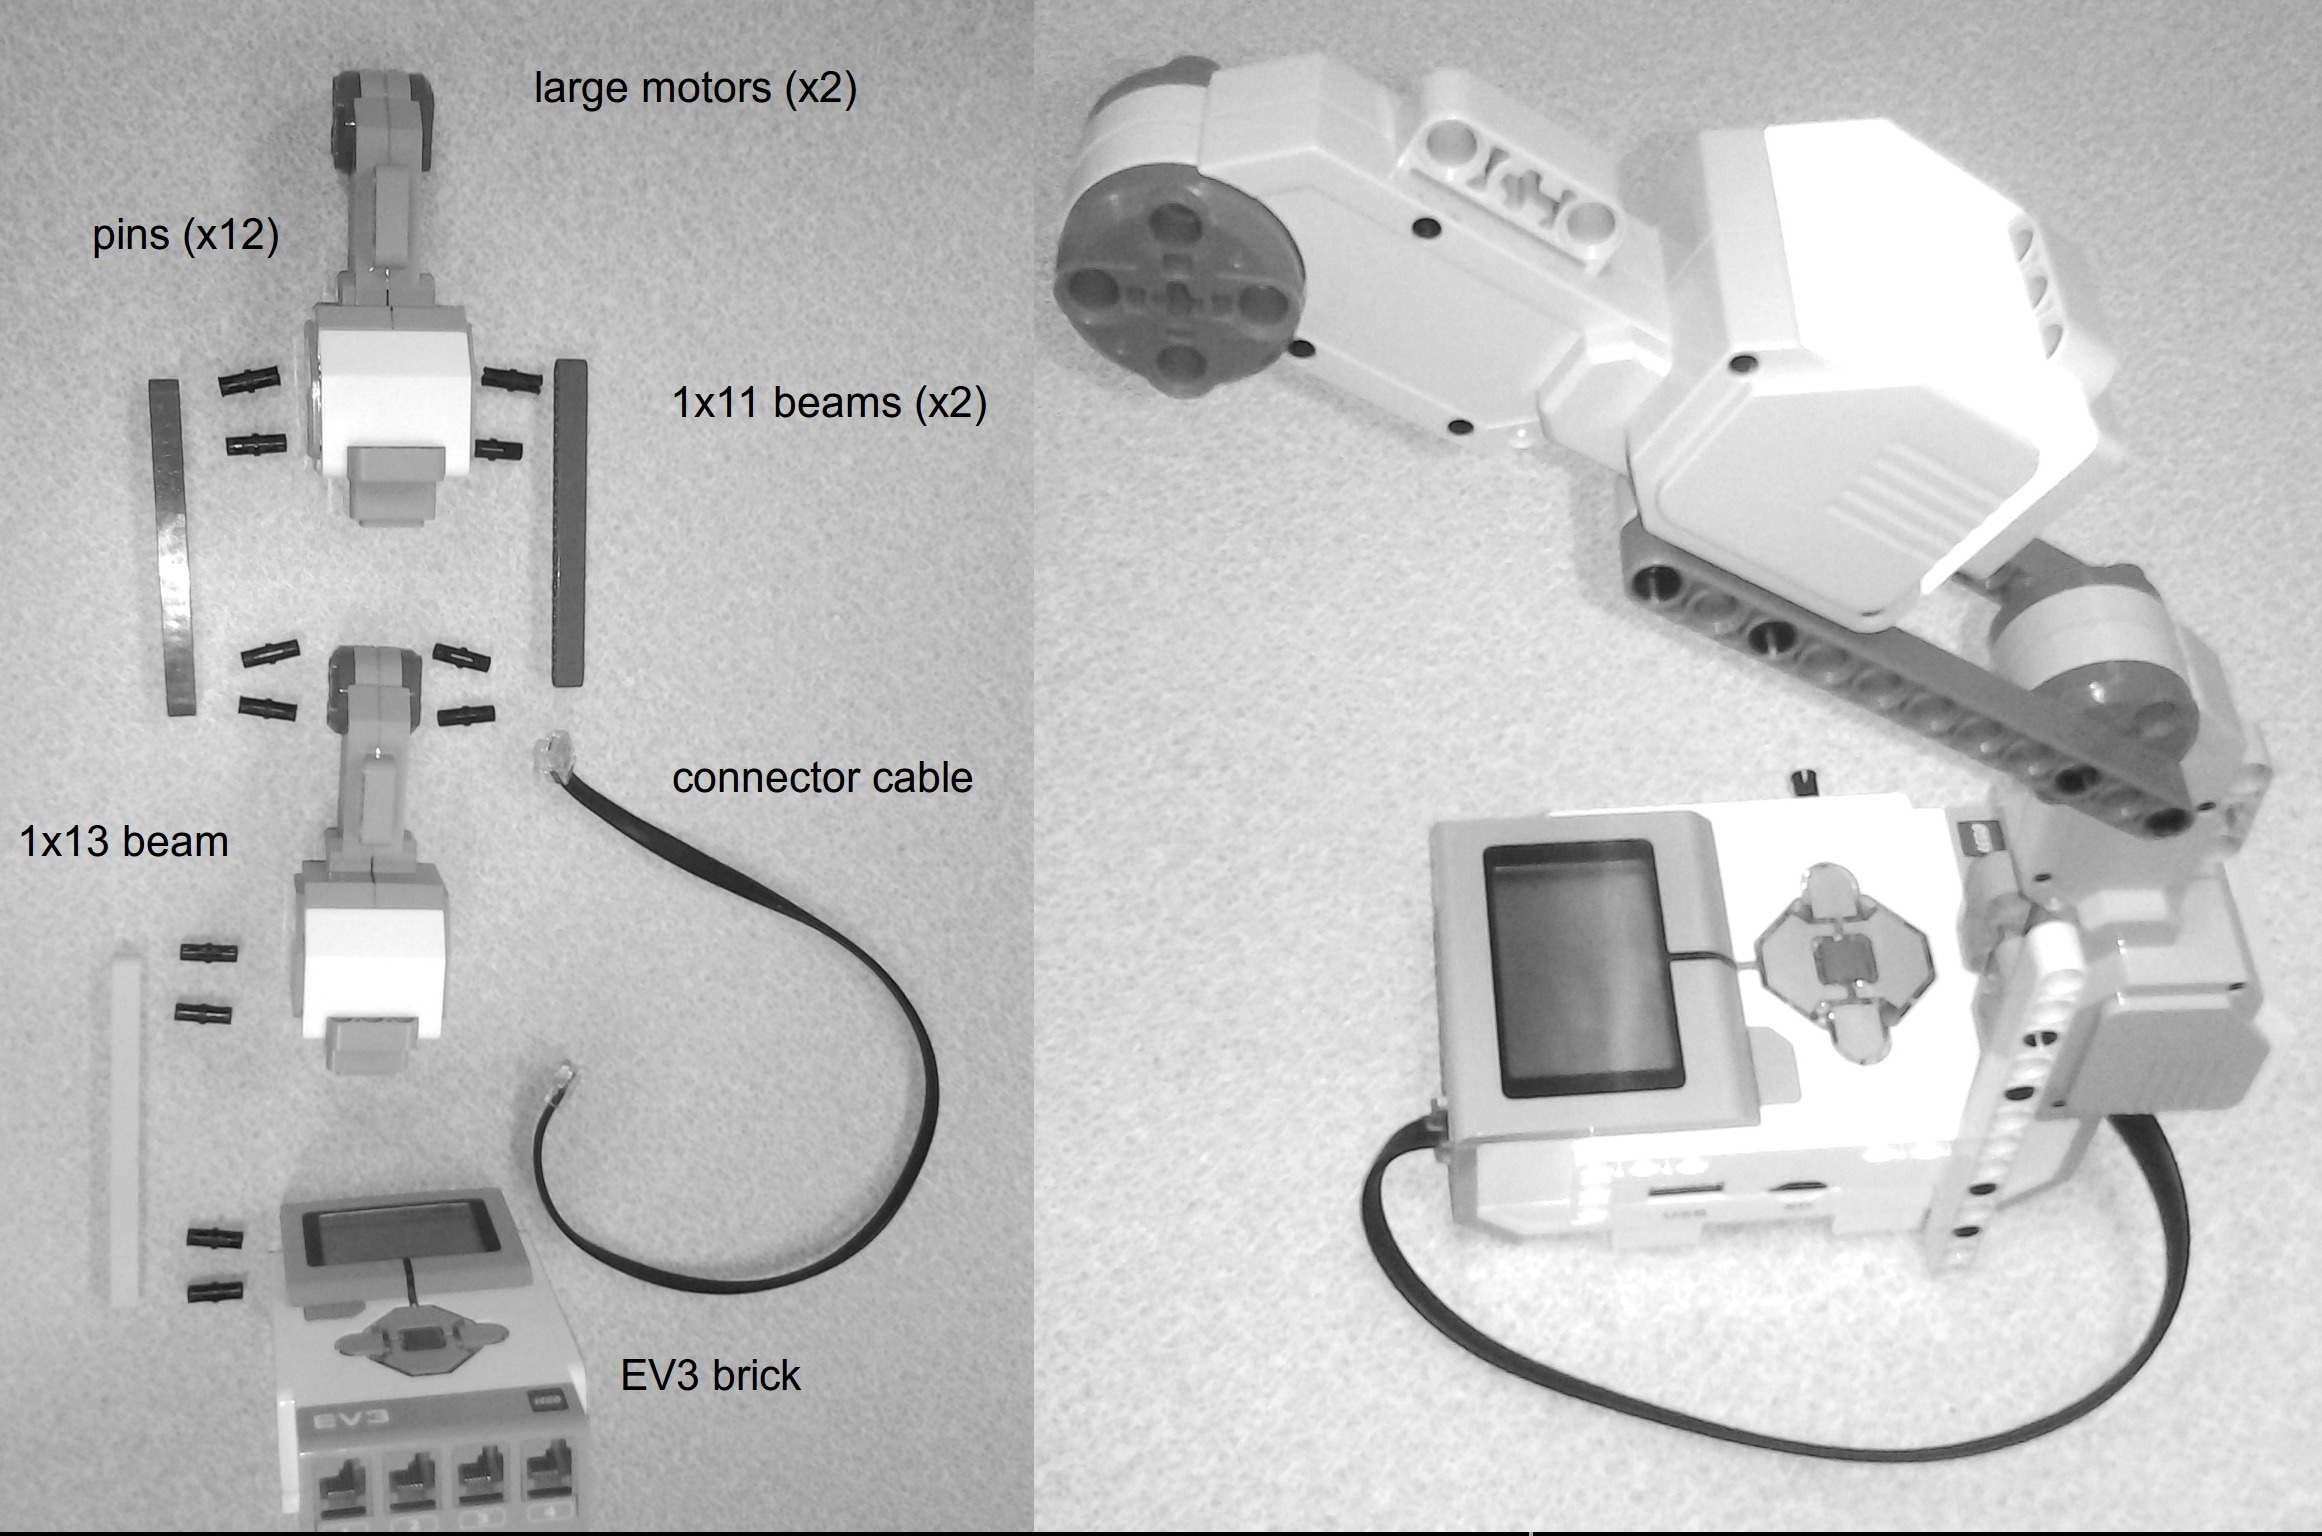
\includegraphics[width=18cm]{figures/lego_labelled}
\end{center}
 \textbf{\refstepcounter{figure}\label{fig:lego} Figure \arabic{figure}.}{ A
     simple physical robot embodiment for calibrating the minimal simulation.
     All components come with the Lego Mindstorms EV3 kit, and are shown on
     the left (2 large motors; 2 1x11 beams; 1 1x13 beam; 12 pins;
     1 EV3 brick; 1 connector cable).
     To rotate the central motor to the desired position $q$, enough force
 must be added to $u$ to counteract the weight of the second unused motor.}
\end{figure}

\begin{figure}[h!]
\begin{center}
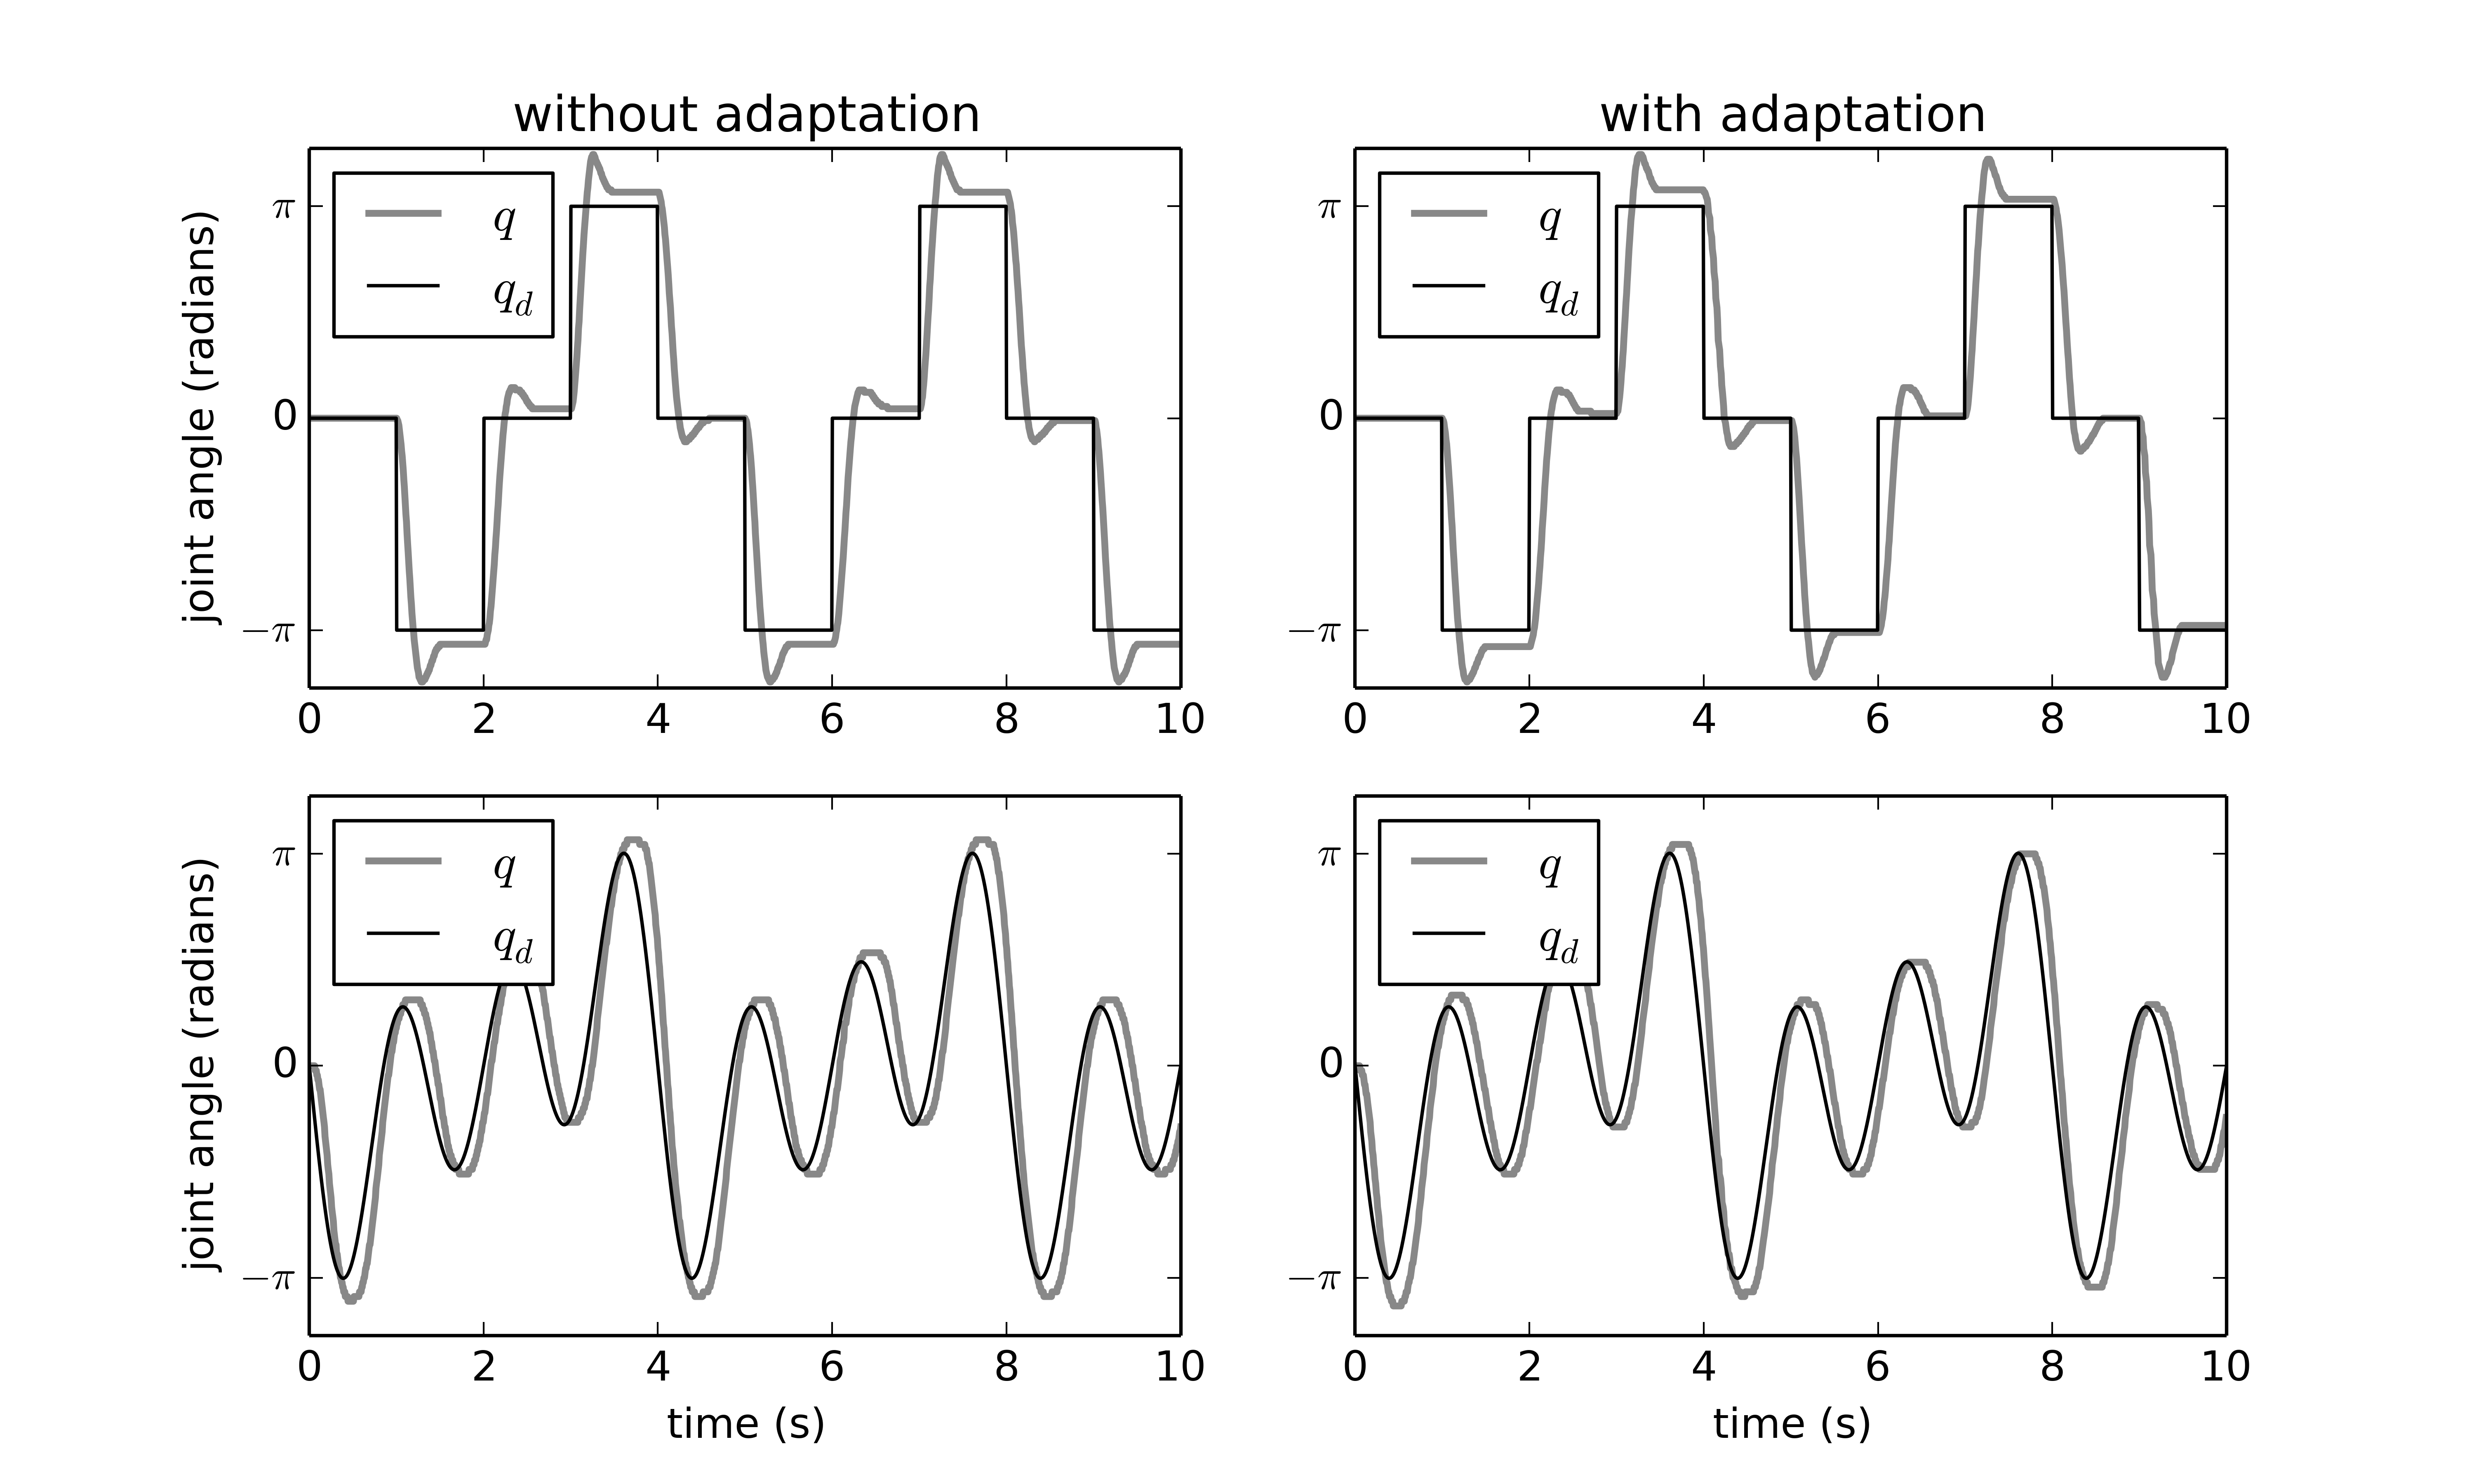
\includegraphics[width=18cm]{figures/fig_ev3}
\end{center}
 \textbf{\refstepcounter{figure}\label{fig:ev3} Figure \arabic{figure}.}{ Adaptive control of the EV3 lego robot used for calibrating the minimal simulation.
 The effects of adaptation over two different desired trajectories are shown.  Without adaptation, the joints $q$ do not reach the desired $q_d$ when $q_d$ is large (which
 is when the external force is largest).  With adaptation, $q$ is closer to $q_d$ after about 5 seconds, showing that the system has quickly learned to compensate.
 Points in time where the improvement is clearest are circled.}
\end{figure}

\begin{figure}[h!]
\begin{center}
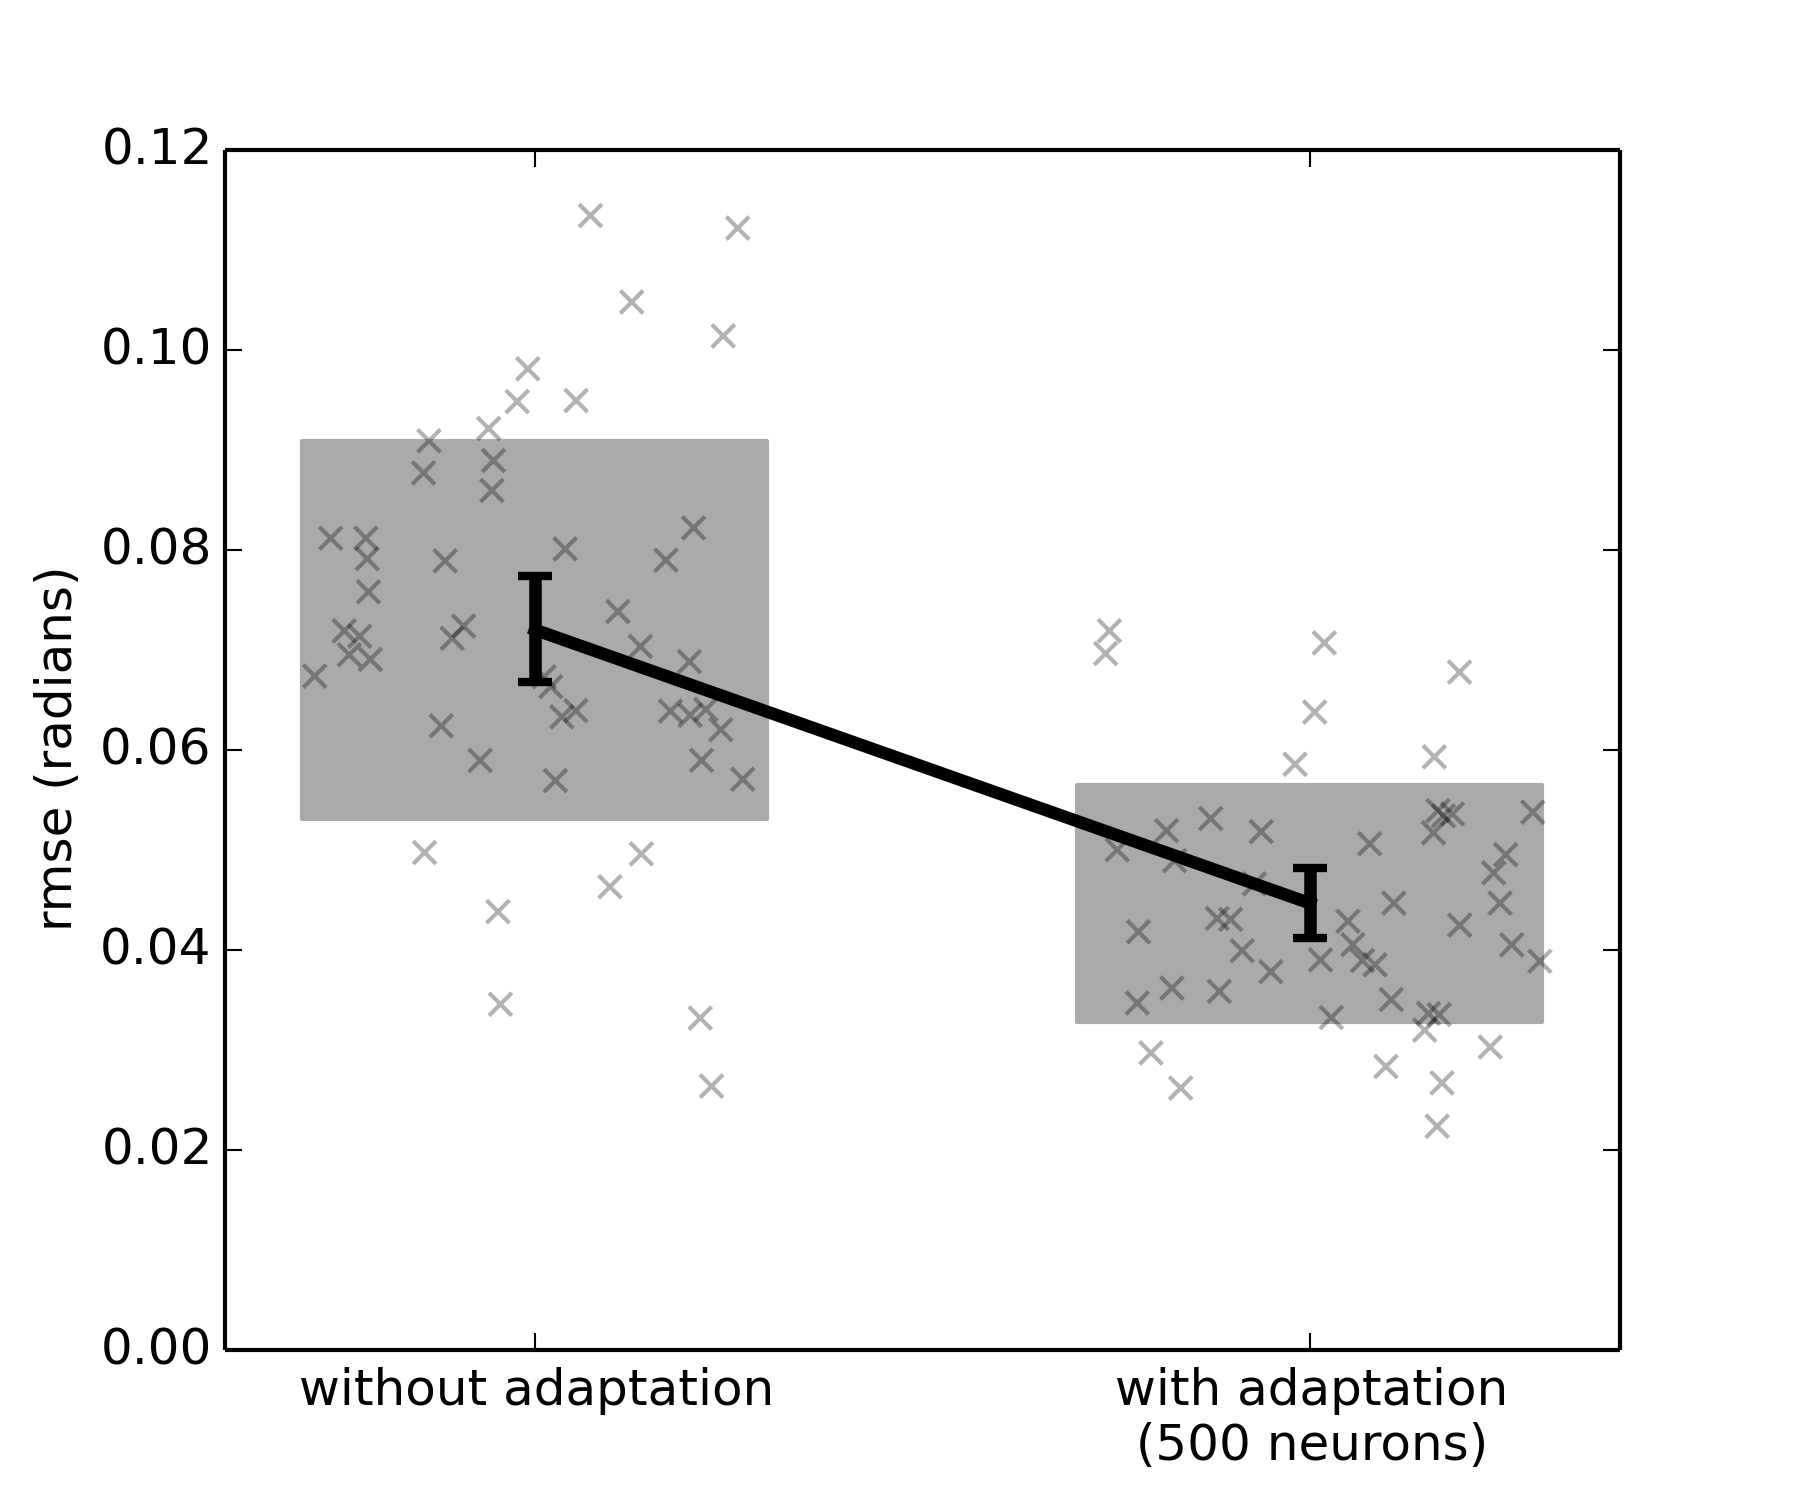
\includegraphics[width=9cm]{figures/plot_ev3}
\end{center}
 \textbf{\refstepcounter{figure}\label{fig:ev3runs} Figure \arabic{figure}.}{ The effect
     of adaptive control on a single-joint lego robot (Figure \ref{fig:lego}).
     Each run uses a randomly generated desired trajectory $q_d(t)$ over
     20 seconds, and root-mean-squared-error is computed over the last
     10 seconds only.  The adaptive algorithm provides a significant improvement
     ($p<0.05$; two-tailed t-test; 50 samples).
     Scatterplots show individual runs (with random jitter on the x-axis
     to avoid overlap), the 
     shaded area is the mean plus or minus the standard deviation, and the 95\% confidence interval of the mean is shown.}
\end{figure}

\begin{figure}[h!]
\begin{center}
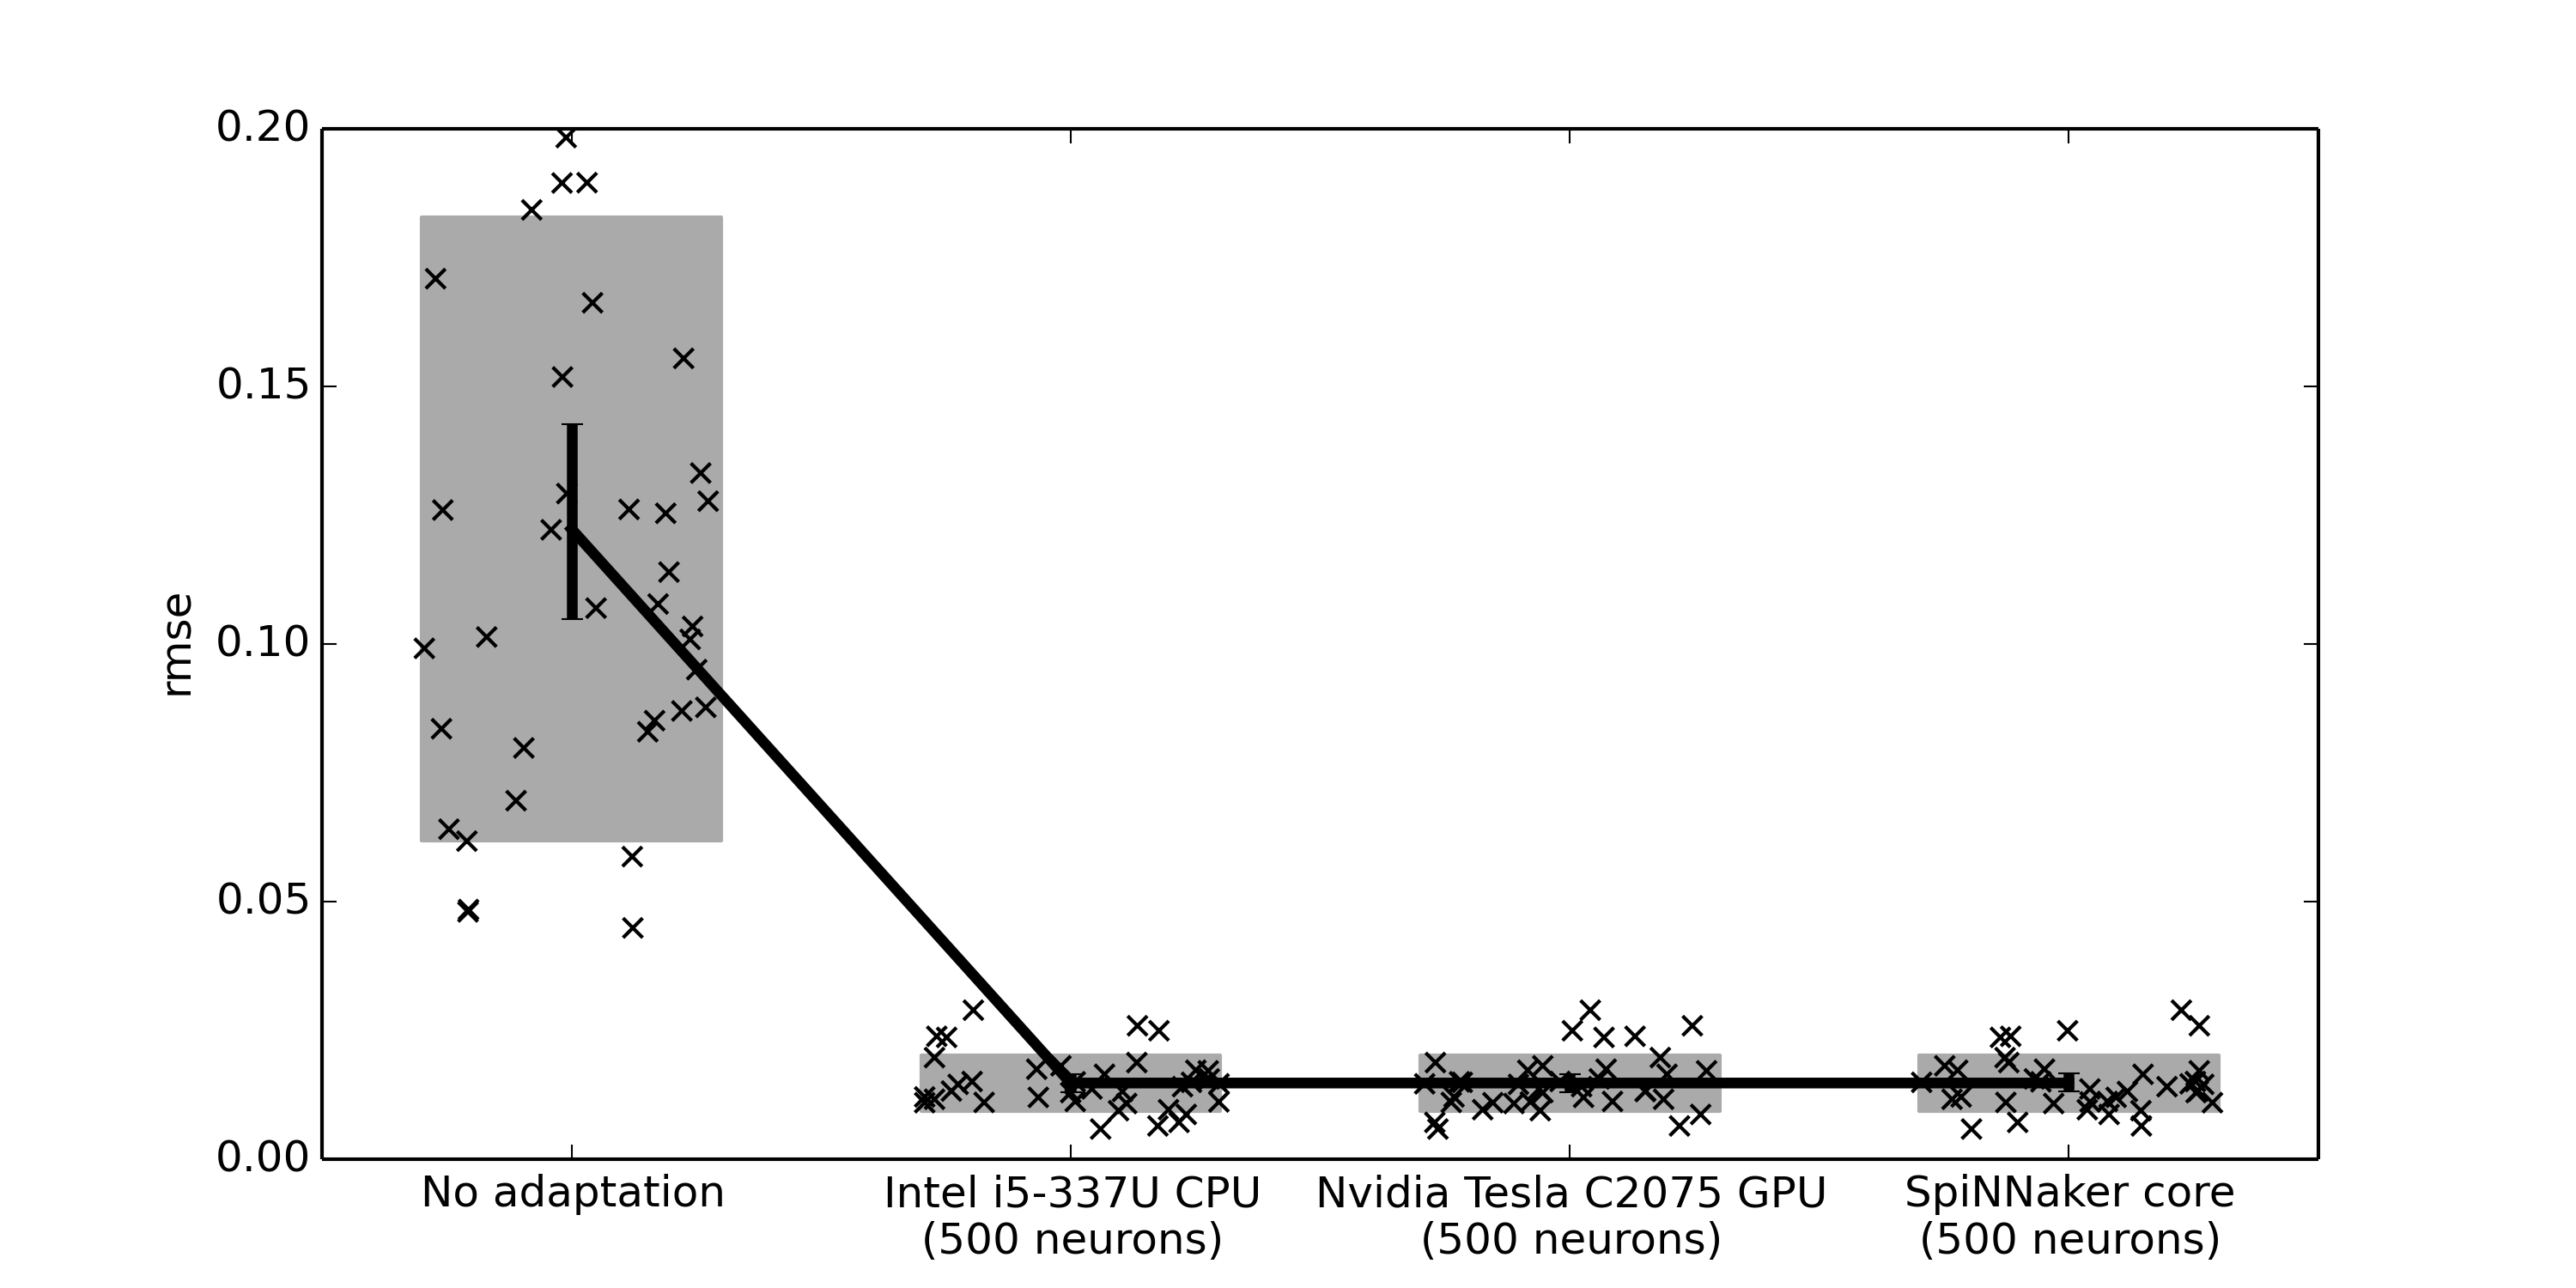
\includegraphics[width=18cm]{figures/plot_basic}
\end{center}
 \textbf{\refstepcounter{figure}\label{fig:analysis_basic} Figure \arabic{figure}.}{ Benchmark results comparing three hardware systems.
     Each system is running 500 neurons.  The hardware do not statistically
     significantly differ, but are all statistically significant improvements 
     over no adaptation ($p<0.05$; two-tailed t-test with Bonferroni correction; 400 samples per condition).
     Scatterplots show individual runs (with random jitter on the x-axis
     to avoid overlap), the 
     shaded area is the mean plus or minus the standard deviation, and the 95\% confidence interval of the mean is shown.}
\end{figure}

\begin{figure}[h!]
\begin{center}
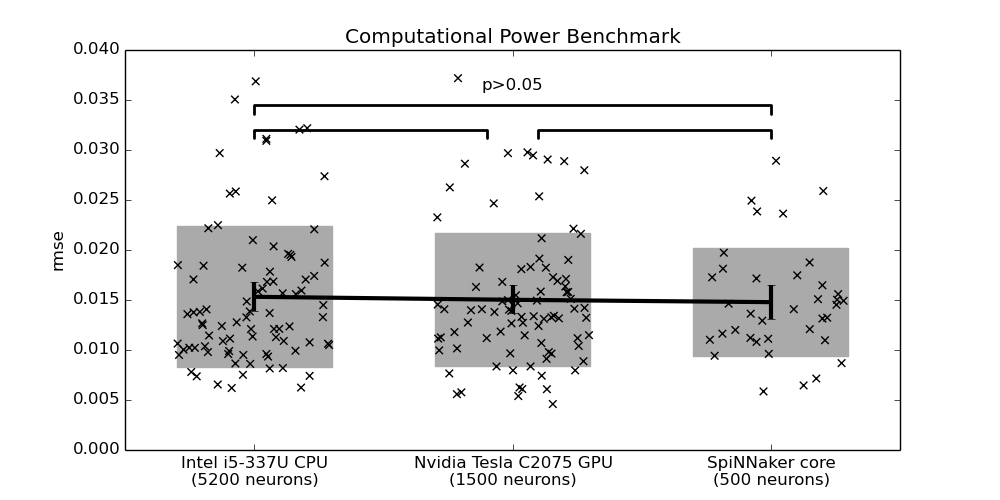
\includegraphics[width=18cm]{figures/plot_compute}
\end{center}
 \textbf{\refstepcounter{figure}\label{fig:analysis_compute} Figure \arabic{figure}.}{ Benchmark results comparing three hardware systems
     in terms of their performance when running as many neurons as they are capable of in real time.  Scatterplots show individual runs (with random
     jitter on the x-axis to avoid overlap), the 
     shaded area is the mean plus or minus the standard deviation, and the 95\% confidence interval of the mean is shown.  In this case,
 there is no statistical difference between the three hardware systems ($p>0.05$; two-tailed t-test with Bonferroni correction; 400 samples per condition).}
\end{figure}

\begin{figure}[h!]
\begin{center}
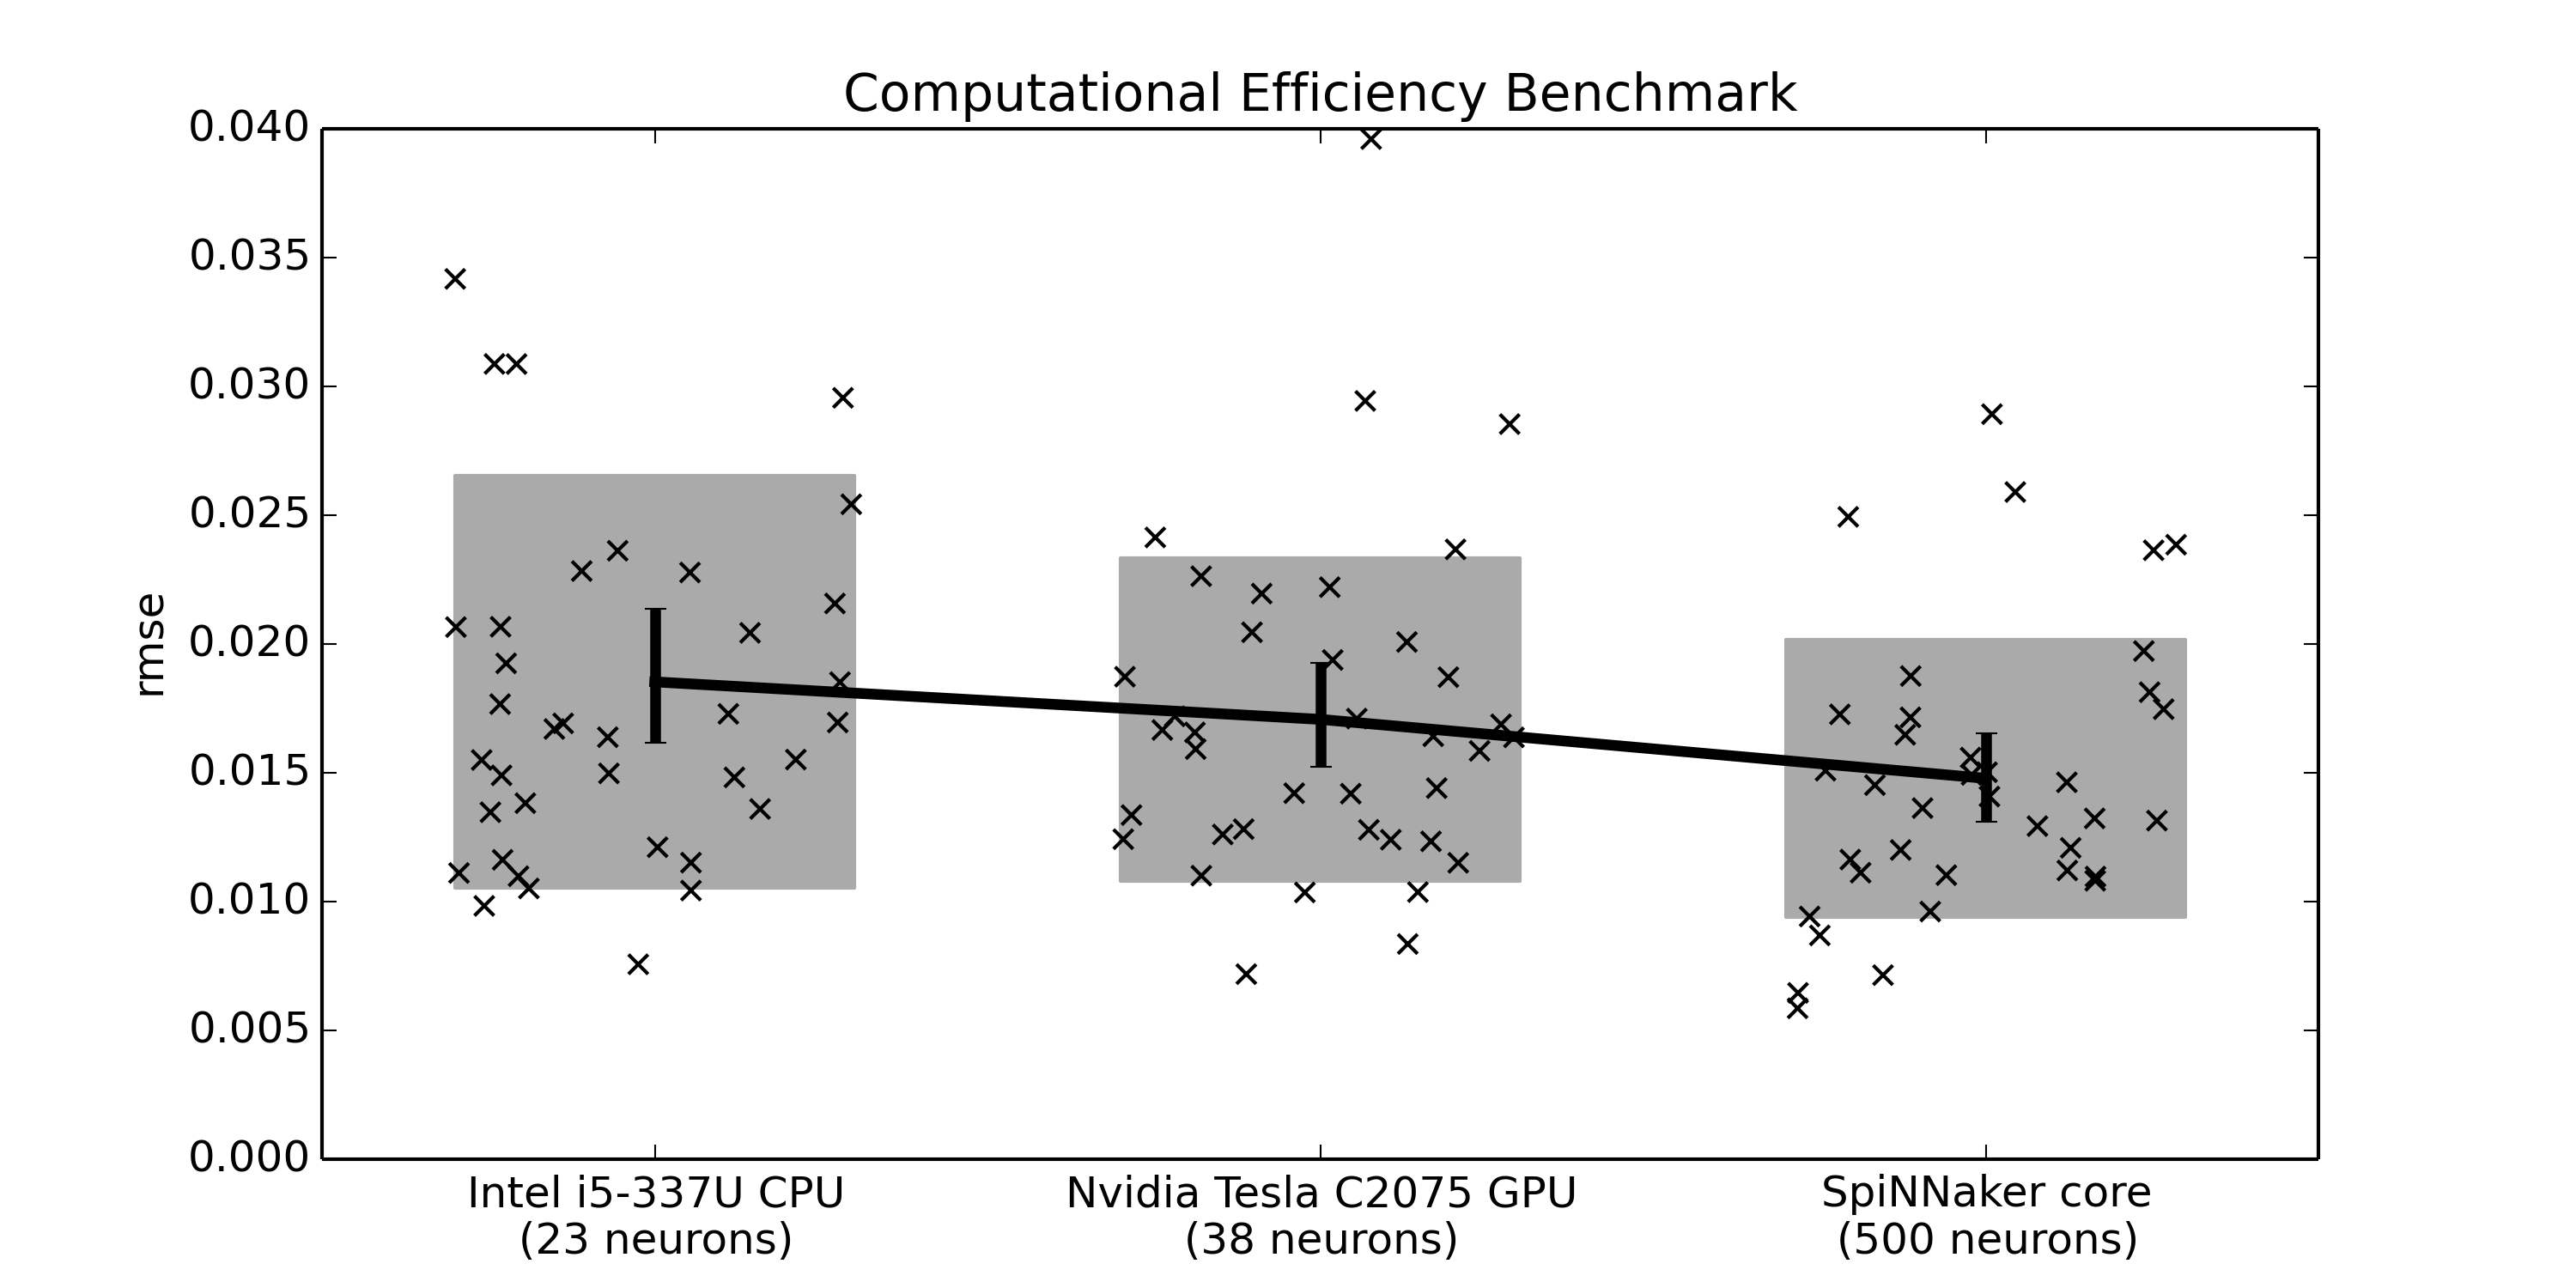
\includegraphics[width=18cm]{figures/plot_power}
\end{center}
 \textbf{\refstepcounter{figure}\label{fig:analysis_power} Figure \arabic{figure}.}{ Benchmark results comparing three hardware systems
     in terms of their performance when running as many neurons as they are capable of per 0.1 Watt of power consumption.  Scatterplots show individual runs (with random jitter on the x-axis to avoid overlap), the 
     shaded area is the mean plus or minus the standard deviation, and the 95\% confidence interval of the mean is shown.  
 All differences are statistically significant ($p<0.05$; two-tailed t-test with Bonferroni correction; 400 samples per condition).}
\end{figure}

\begin{figure}[h!]
\begin{center}
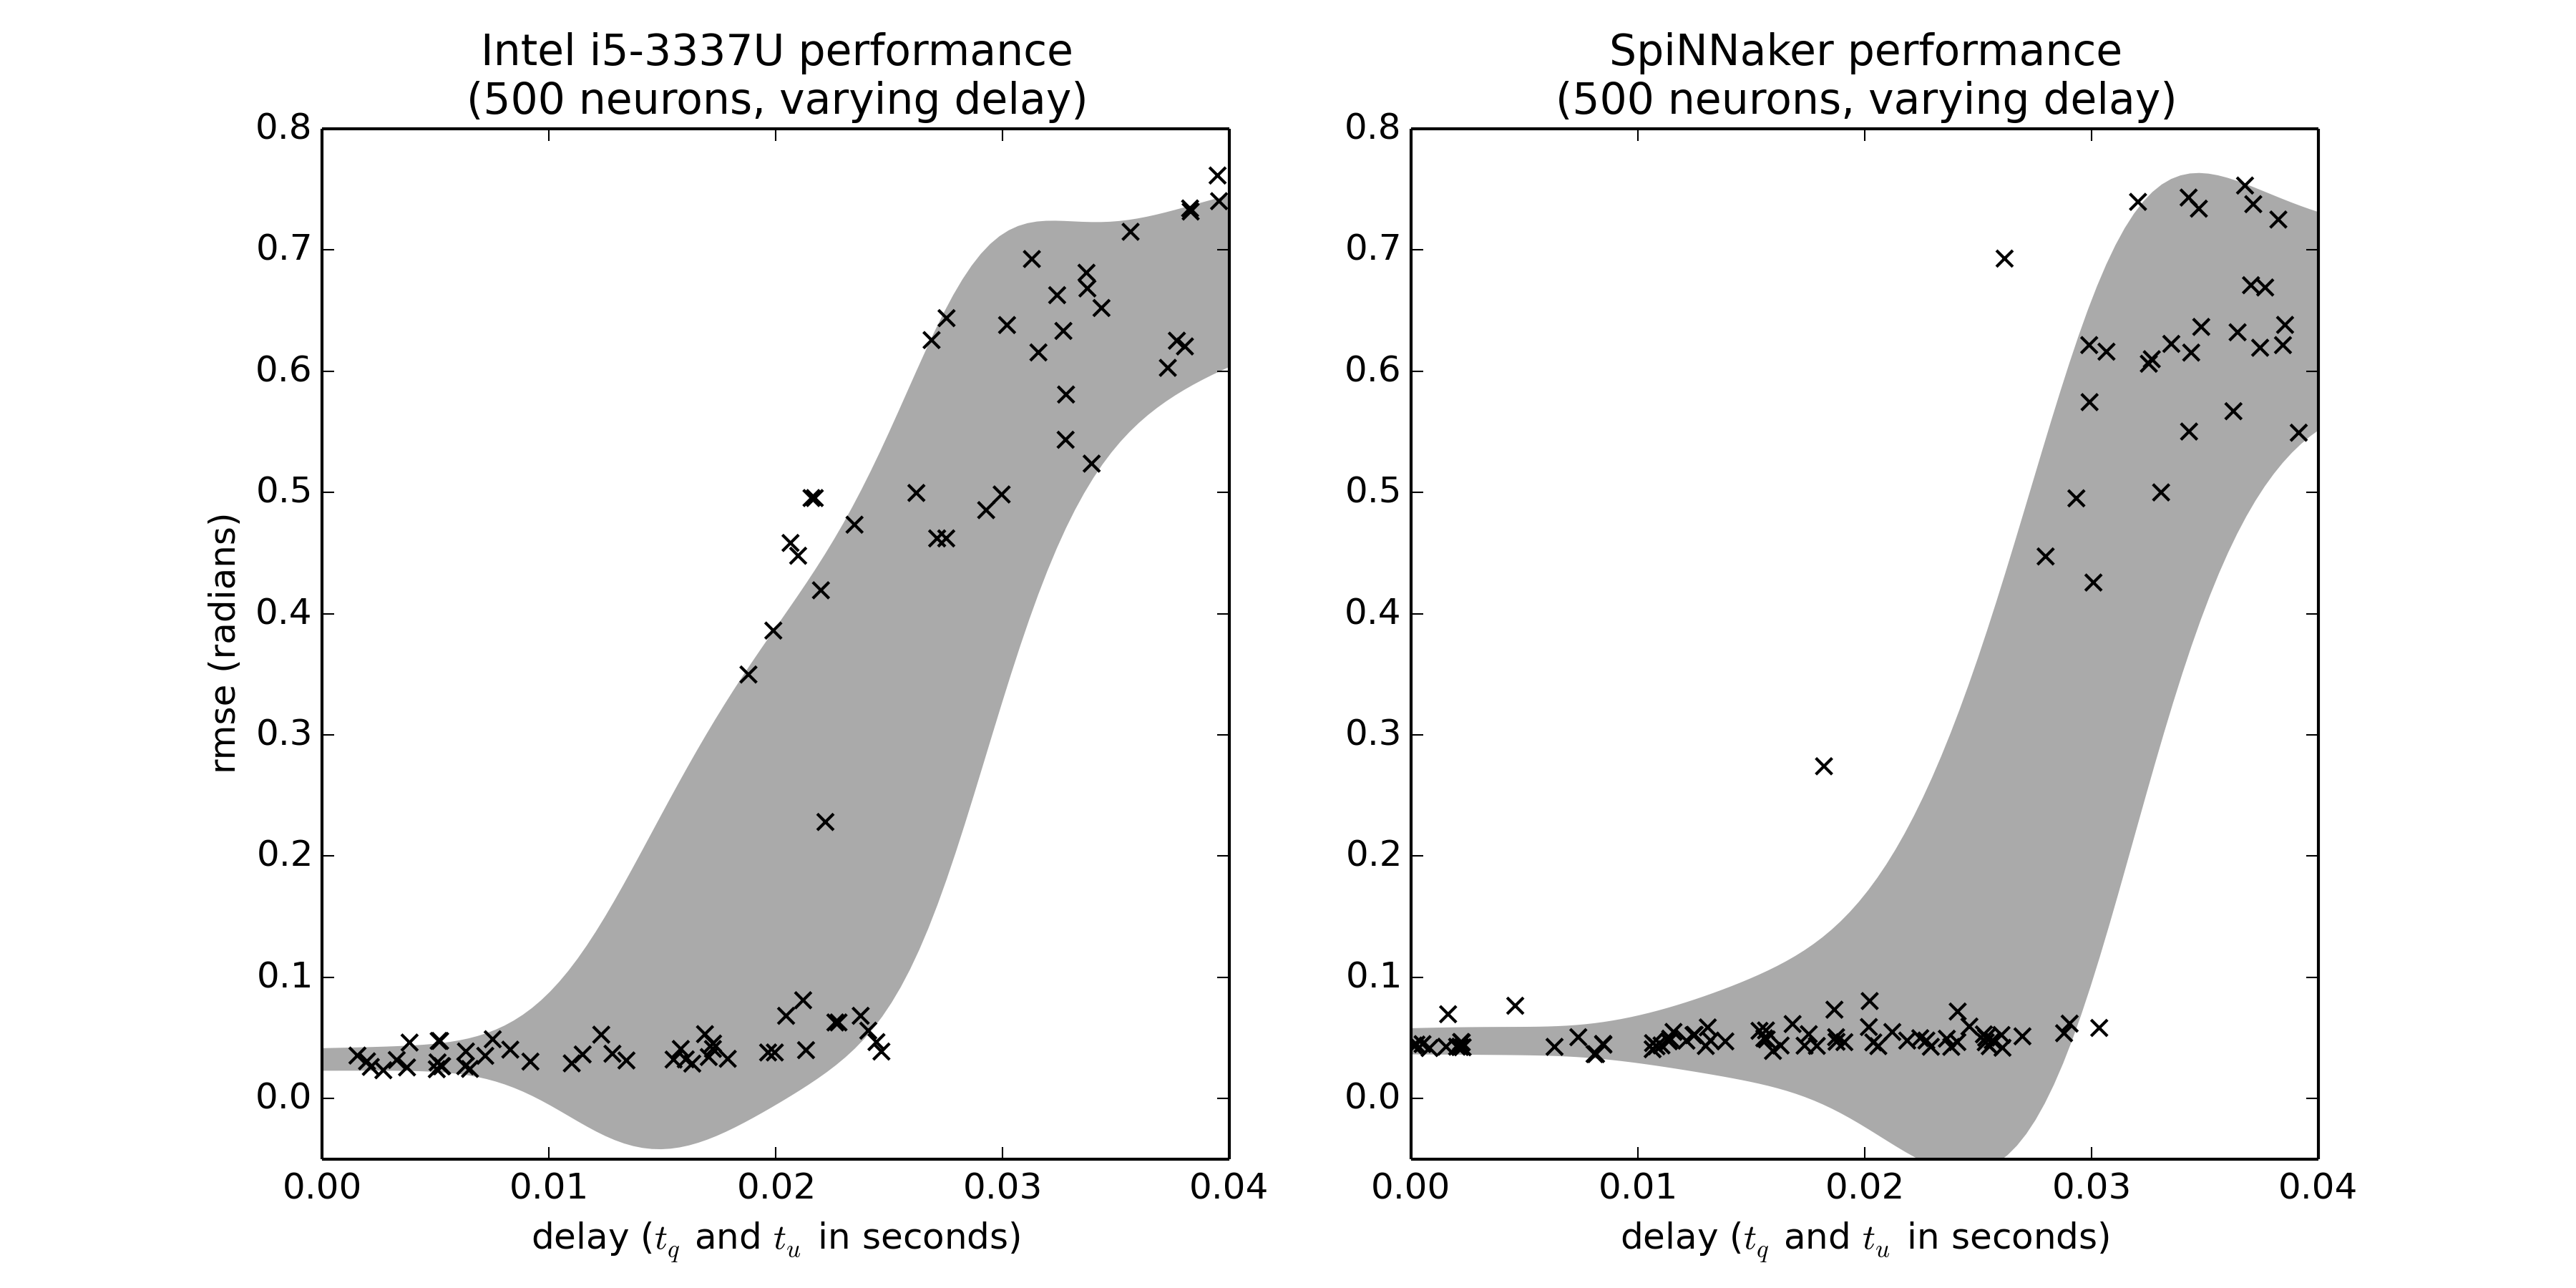
\includegraphics[width=18cm]{figures/plot_delay}
\end{center}
 \textbf{\refstepcounter{figure}\label{fig:analysis_delay} Figure \arabic{figure}.}{ Benchmark results comparing the effects
     of communication delay for the CPU and SpiNNaker systems.  The delays $t_q$ and $t_u$ are randomly varied.  Shaded
 area is the mean plus or minus one standard deviation, smoothed with a Gaussian kernel of $\sigma=0.005$.}
\end{figure}

\begin{figure}[h!]
\begin{center}
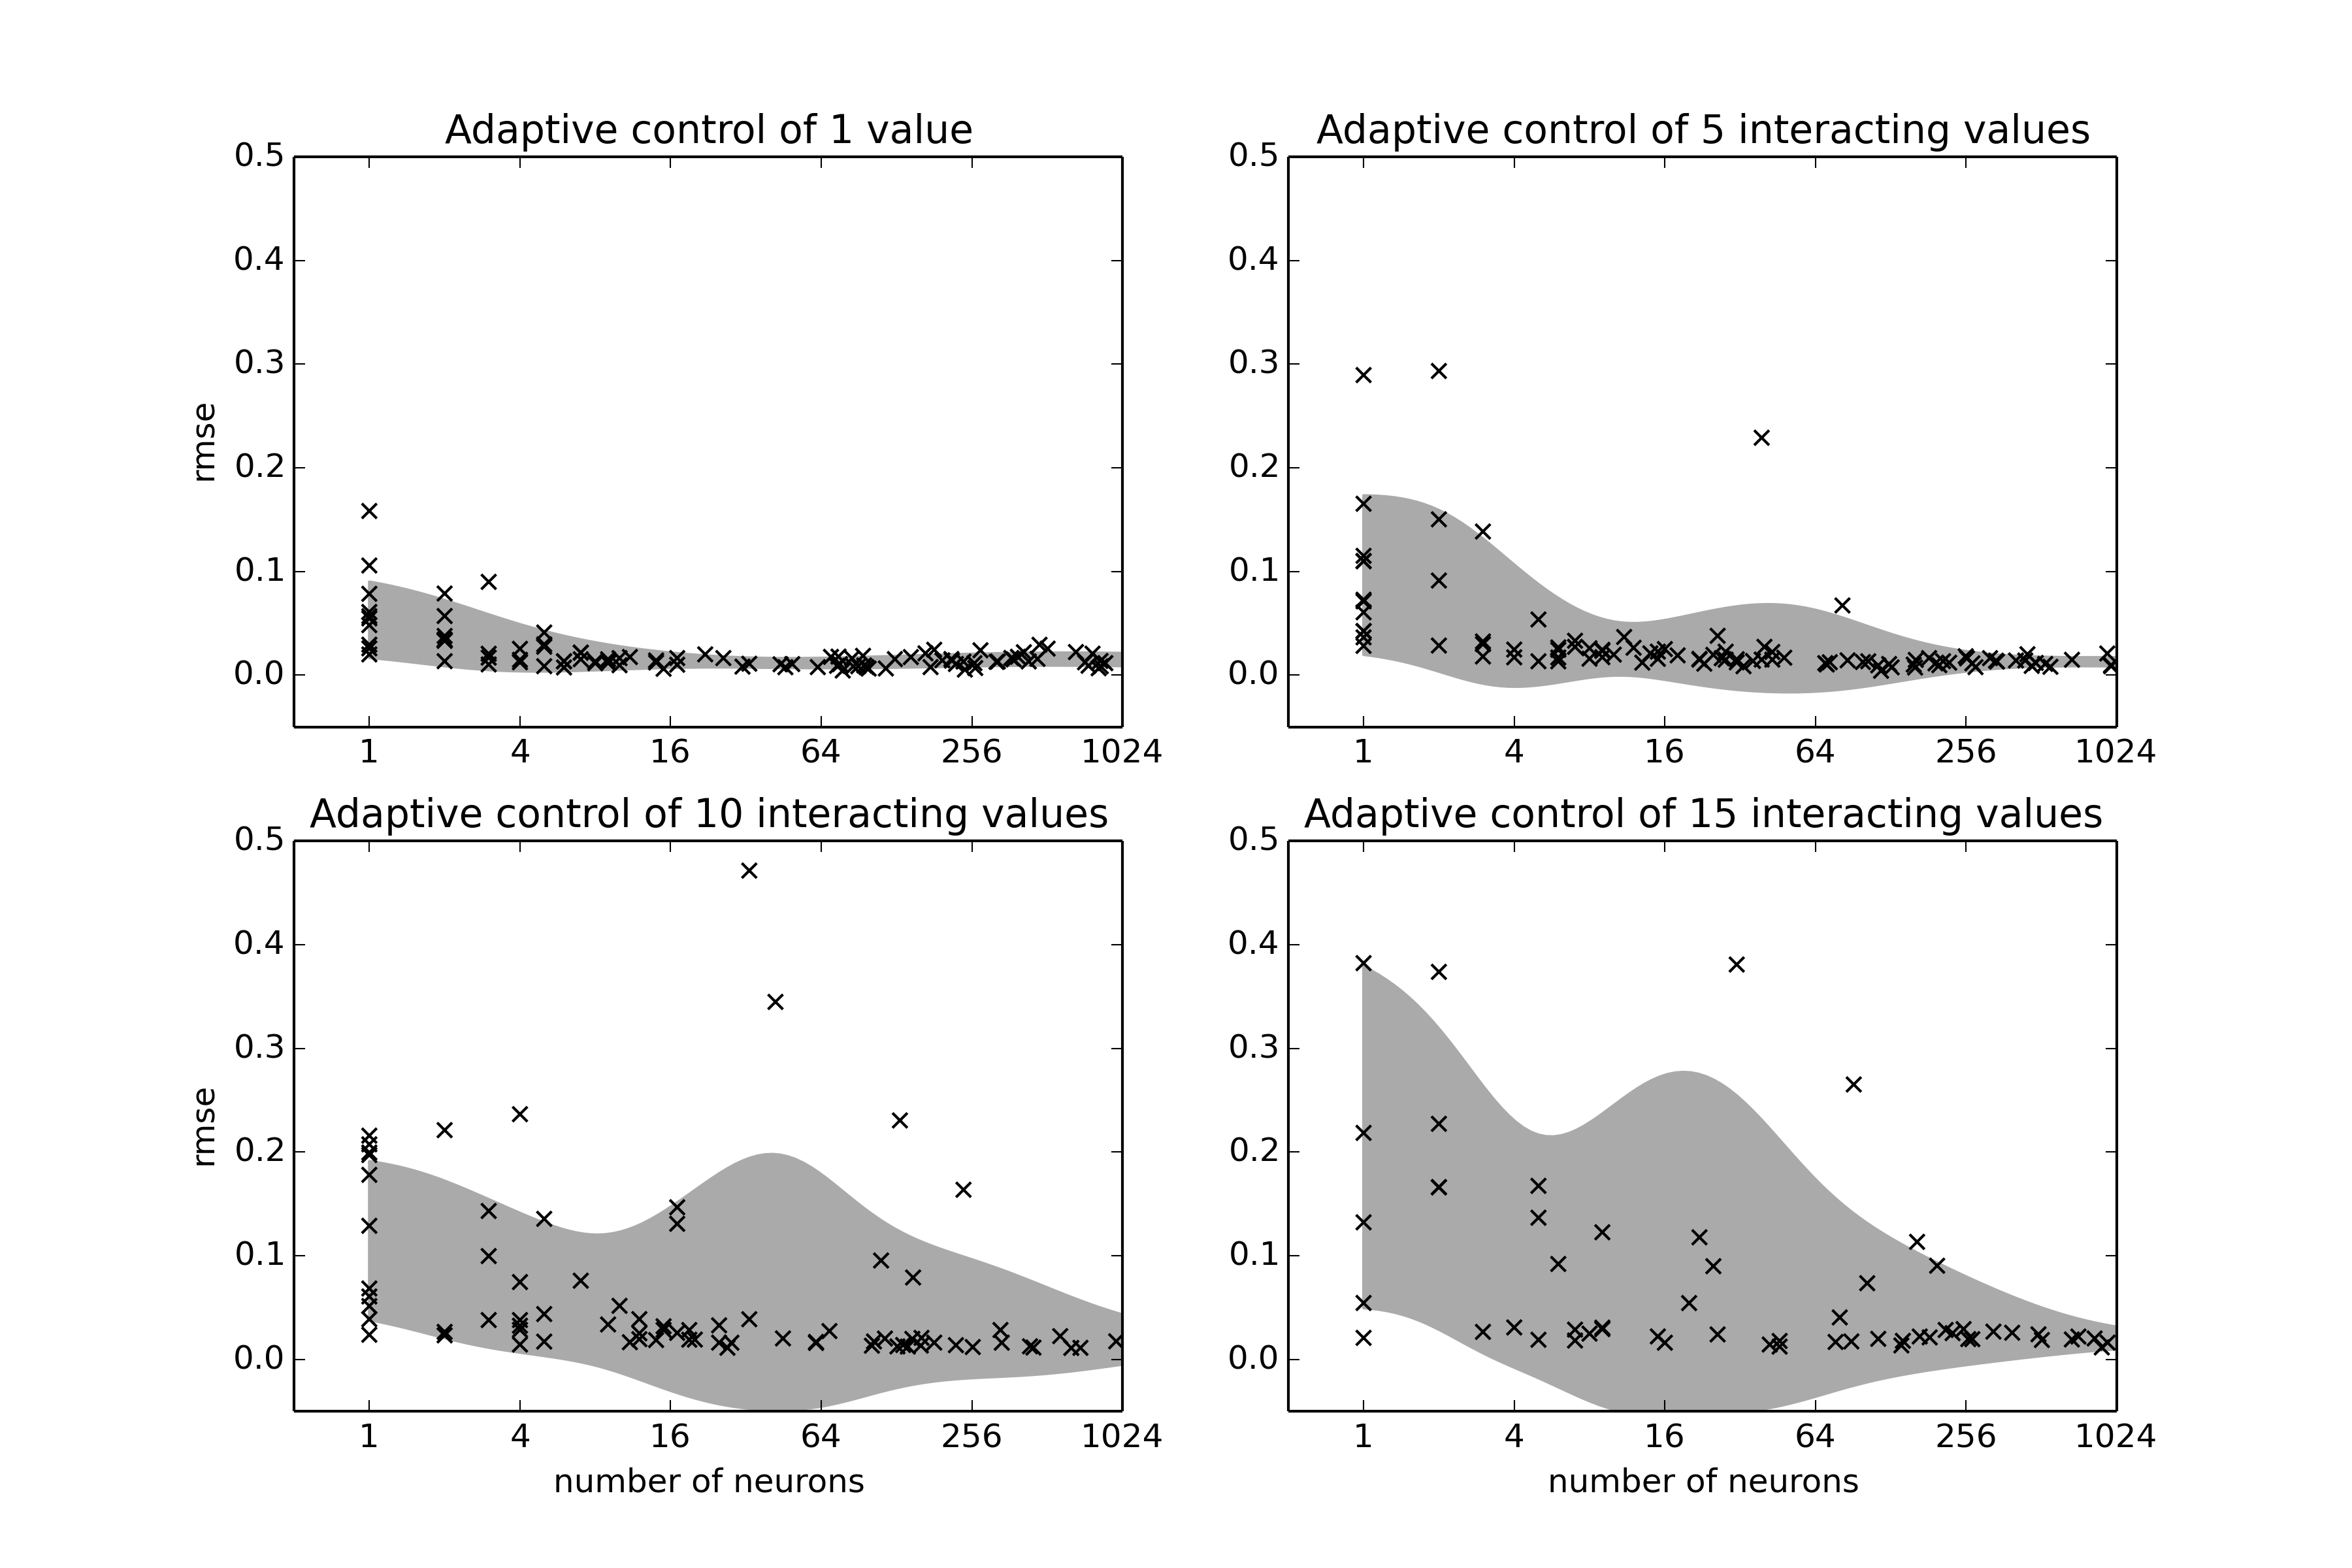
\includegraphics[width=18cm]{figures/plot_vary_neurons}
\end{center}
 \textbf{\refstepcounter{figure}\label{fig:analysis_neurons_cpu} Figure \arabic{figure}.}{ Benchmark results examining the relationship
     between number of neurons and the number of simulated joints $N$.  The
     benchmark was run on the Intel i5-3337U CPU.  Shaded
 area is the mean plus or minus one standard deviation, smoothed with a Gaussian kernel of $\sigma=1$ in the $log_2$ domain.}
\end{figure}
%\begin{figure}
%\begin{center}
%
\includegraphics[width=10cm]{logo2}% This is an *.eps file
%\end{center}
%\textbf{\refstepcounter{figure}\label{fig:02} Figure \arabic{figure}.}{ Enter the caption for your figure here.  Repeat as  necessary for each of your figures }
%\end{figure}

%%% If you don't add the figures in the LaTeX files, please upload them when submitting the article.

%%% Frontiers will add the figures at the end of the provisional pdf automatically %%%

%%% The use of LaTeX coding to draw Diagrams/Figures/Structures should be avoided. They should be external callouts including graphics.

\end{document}
